%%================================================
%% Filename: chap02.tex
%% Encoding: UTF-8
%% Author: 苏峻锋
%% Created: 2024-02-26
%% Last modified: 2024-02-28
%%================================================
\chapter{相关理论及技术研究}

\section{服务器集群}

\subsection{服务器集群定义}

服务器集群,又称集群(Cluster),是由多台服务器以线性方式相连而成的一个整体系统。在集群中,每台服务器都被视为一个节点,这些节点之间能够相互通信、协同工作,共同构建出一个高性能的服务器系统\cite{kanellopoulos2022dynamic}。当客户端(Client)发送请求时,集群内的各个服务节点会协同处理这些请求,同时通过数据库或消息队列等存储方式在节点之间共享业务数据。
从客户端的视角来看,整个服务器集群被视为一个统一的整体,集群对外隐藏了各服务节点间的通信细节,呈现出逻辑上的一致性。
\begin{figure}[ht]
	\centering
	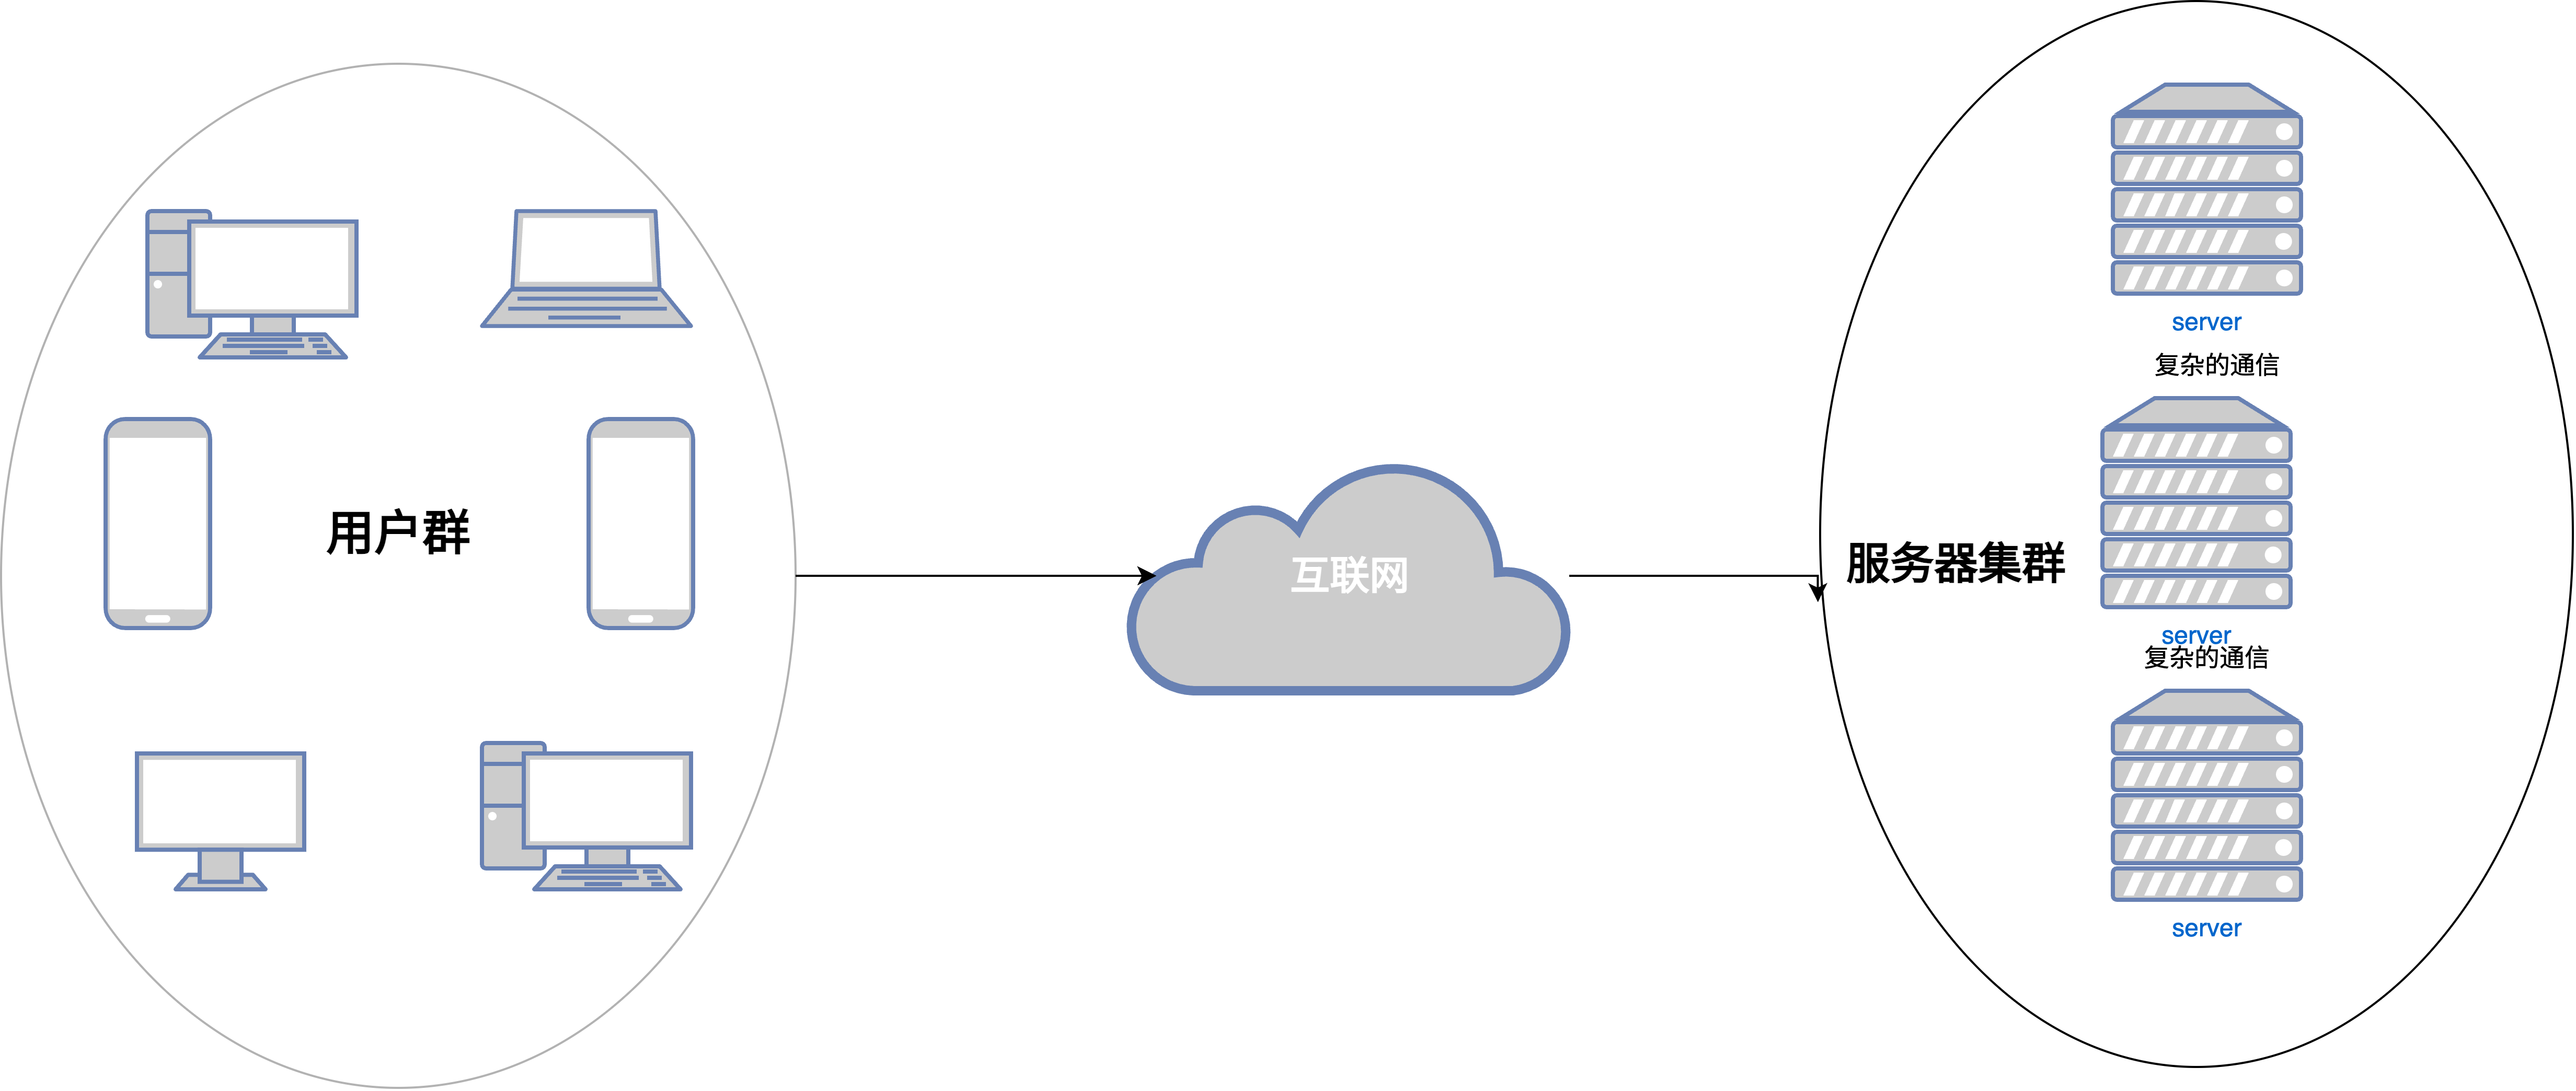
\includegraphics[width=\textwidth]{figures/cluster-and-client.png}
	\caption{服务器集群与客户端}
\end{figure}

\subsection{服务器集群的架构优势}

(1)高性能

服务器集群通过协调不同物理硬件性能的服务器,在服务器服务节点处理客户端的请求时,尤其是高并发的场景下,相比于
单个服务器而言,集群架构表现了优越的性能。这种优越的性能不仅仅是不同性能设备能力的叠加,更是因为通信细节的互相协作,紧密联系造就的。

(2)高可用

服务器集群的高可用性主要体现在其容灾和故障转移能力上\cite{刘金秀2019基于}。对于大型企业应用而言,单个服务器因处理器负载过高或其他原因导致的重启或崩溃是不可接受的。
服务器集群能够有效应对单点故障引发的问题。即便集群中某个服务节点出现异常,也不会导致整个集群不可用。在这种情况下,集群内其他正常运行的服务节点会立即接管故障节点的工作,确保业务连续性。只有当集群内所有服务节点同时发生故障时,集群才会停止提供服务。

(3)可伸缩性

可伸缩性实现了对服务器节点灵活管理,并且用户对此并无感知。在负载比较大的情境下,就需要增加对服务器节点的投入,相反
如果负载比较小的情景下,就可以减少集群内的服务器节点

而本文主要优化的方向就是可伸缩性方面,判断不同情境下可能的负载程度,通过对负载情况的预测,能够对实现可伸缩性较大程度的优化。

\subsection{服务器集群的分类}

服务器集群可以根据多种标准进行分类,采用不同的划分方式会得到不同类型的集群。
除了常见的同构集群外,当前商业领域还大量采用了基于多业务结构划分的异构集群。
从集群的实际功能结构出发,较为常见的集群类型有三种,分别是旨在提升计算性能的高性能计算集群、侧重保障服务稳定性的高可用集群,以及用于优化资源利用率的负载均衡集群\cite{刘卓2017基于Nginx的负载均衡集群设计与实现}。

(1)高性能计算集群

高性能计算集群(HPC集群)是并行计算技术的一个关键研究领域,它主要致力于开发适用于复杂科学问题的多机并行算法及其相应软件工具,以构建能够执行高度复杂运算任务的超级计算系统\cite{xuzongyu}。HPC集群通过并行处理技术,将庞大的计算任务拆分成众多小型子任务,分别在不同的服务器上独立执行,再将每个服务器的计算成果聚合起来,以此获取最终的计算结果。这一过程利用多台计算机的协同工作能力,有效提升了数据处理速度,同时减少了计算所需的时间开销。

随着大数据和人工智能等前沿技术的持续进步,HPC集群的应用范围也在不断拓展。现如今,高性能计算集群已经广泛应用于科学研究的诸多领域中,为处理庞大数据集提供了有力的技术支持。无论是在地质分析、生物医药开发、数据挖掘还是图像识别等领域,HPC集群的作用都不容小觑,它极大地促进了这些科学领域的研究与发展。

(2) 高可用集群

高可用集群顾名思义,即使在高负载、高并发的场景下,可以将该服务器中的服务、资源、IP等转移到另外一台服务器上,从而满足业务的持续性;这两台或多台服务器构成了服务器高可用集群。
简单来说就是京东淘宝24小时不断买买买,微信QQ不断发短信,保证了服务器的不间断运行。然而永远的不间断运行几乎是不可能的,常见的算法并不能彻底处理突然之间的高并发和高负载,比如在双十一期间,某购物网站无法处理突然增加的大量订单
用户刷新造成的DDoS行为,具体衡量标准请看下面这份表。

\noindent\begin{longtblr}[
		caption = {HA衡量标准\cite{信息安全技术信息系统灾难恢复规范}},
	]{
		hlines,
		vlines,
		% colspec={|X[c]|X[c]|X[c]|X[c]|},
	}
	描述             & 通俗叫法 & 可用性级别        & 年度停机时间 \\
	基本可用性          & 2个9  & 99\%         & 87.6小时 \\
	较高可用性          & 3 个9 & 99.9\% 8.8小时          \\
	具有故障自动恢复能力的可用性 & 4 个9 & 99.99\%      & 53 分钟  \\
	极高可用性          & 5 个9 & 99.999\%     & 5 分钟   \\
\end{longtblr}

(3)负载均衡集群

当大量用户并发访问时,负载均衡器将请求转发到不同的机器上,以实现负载均衡。
负载均衡集群由前端的负载均衡器和后端的服务器构成,其中负载均衡器位于客户端和服务器之间。
通过负载均衡调度策略,负载均衡器将负载分发到后端服务器进行处理,从而分散单台服务器的访问压力和存储压力,降低单台服务器宕机对业务造成的影响\cite{吴宝花2020基于}。
为了确保客户端发送的请求能够成功地发送给后端服务器,负载均衡器会判断后端服务器是否正常可用。
如果检测到后端服务器状态正常,则根据相应的负载均衡策略从这些可用的服务器中选择一台服务器处理对应的请求;
但是,如果检测到后端服务器状态异常,则该服务器会被自动剔除,待其恢复正常后再重新加入集群系统。

\begin{figure}[ht]
	\centering
	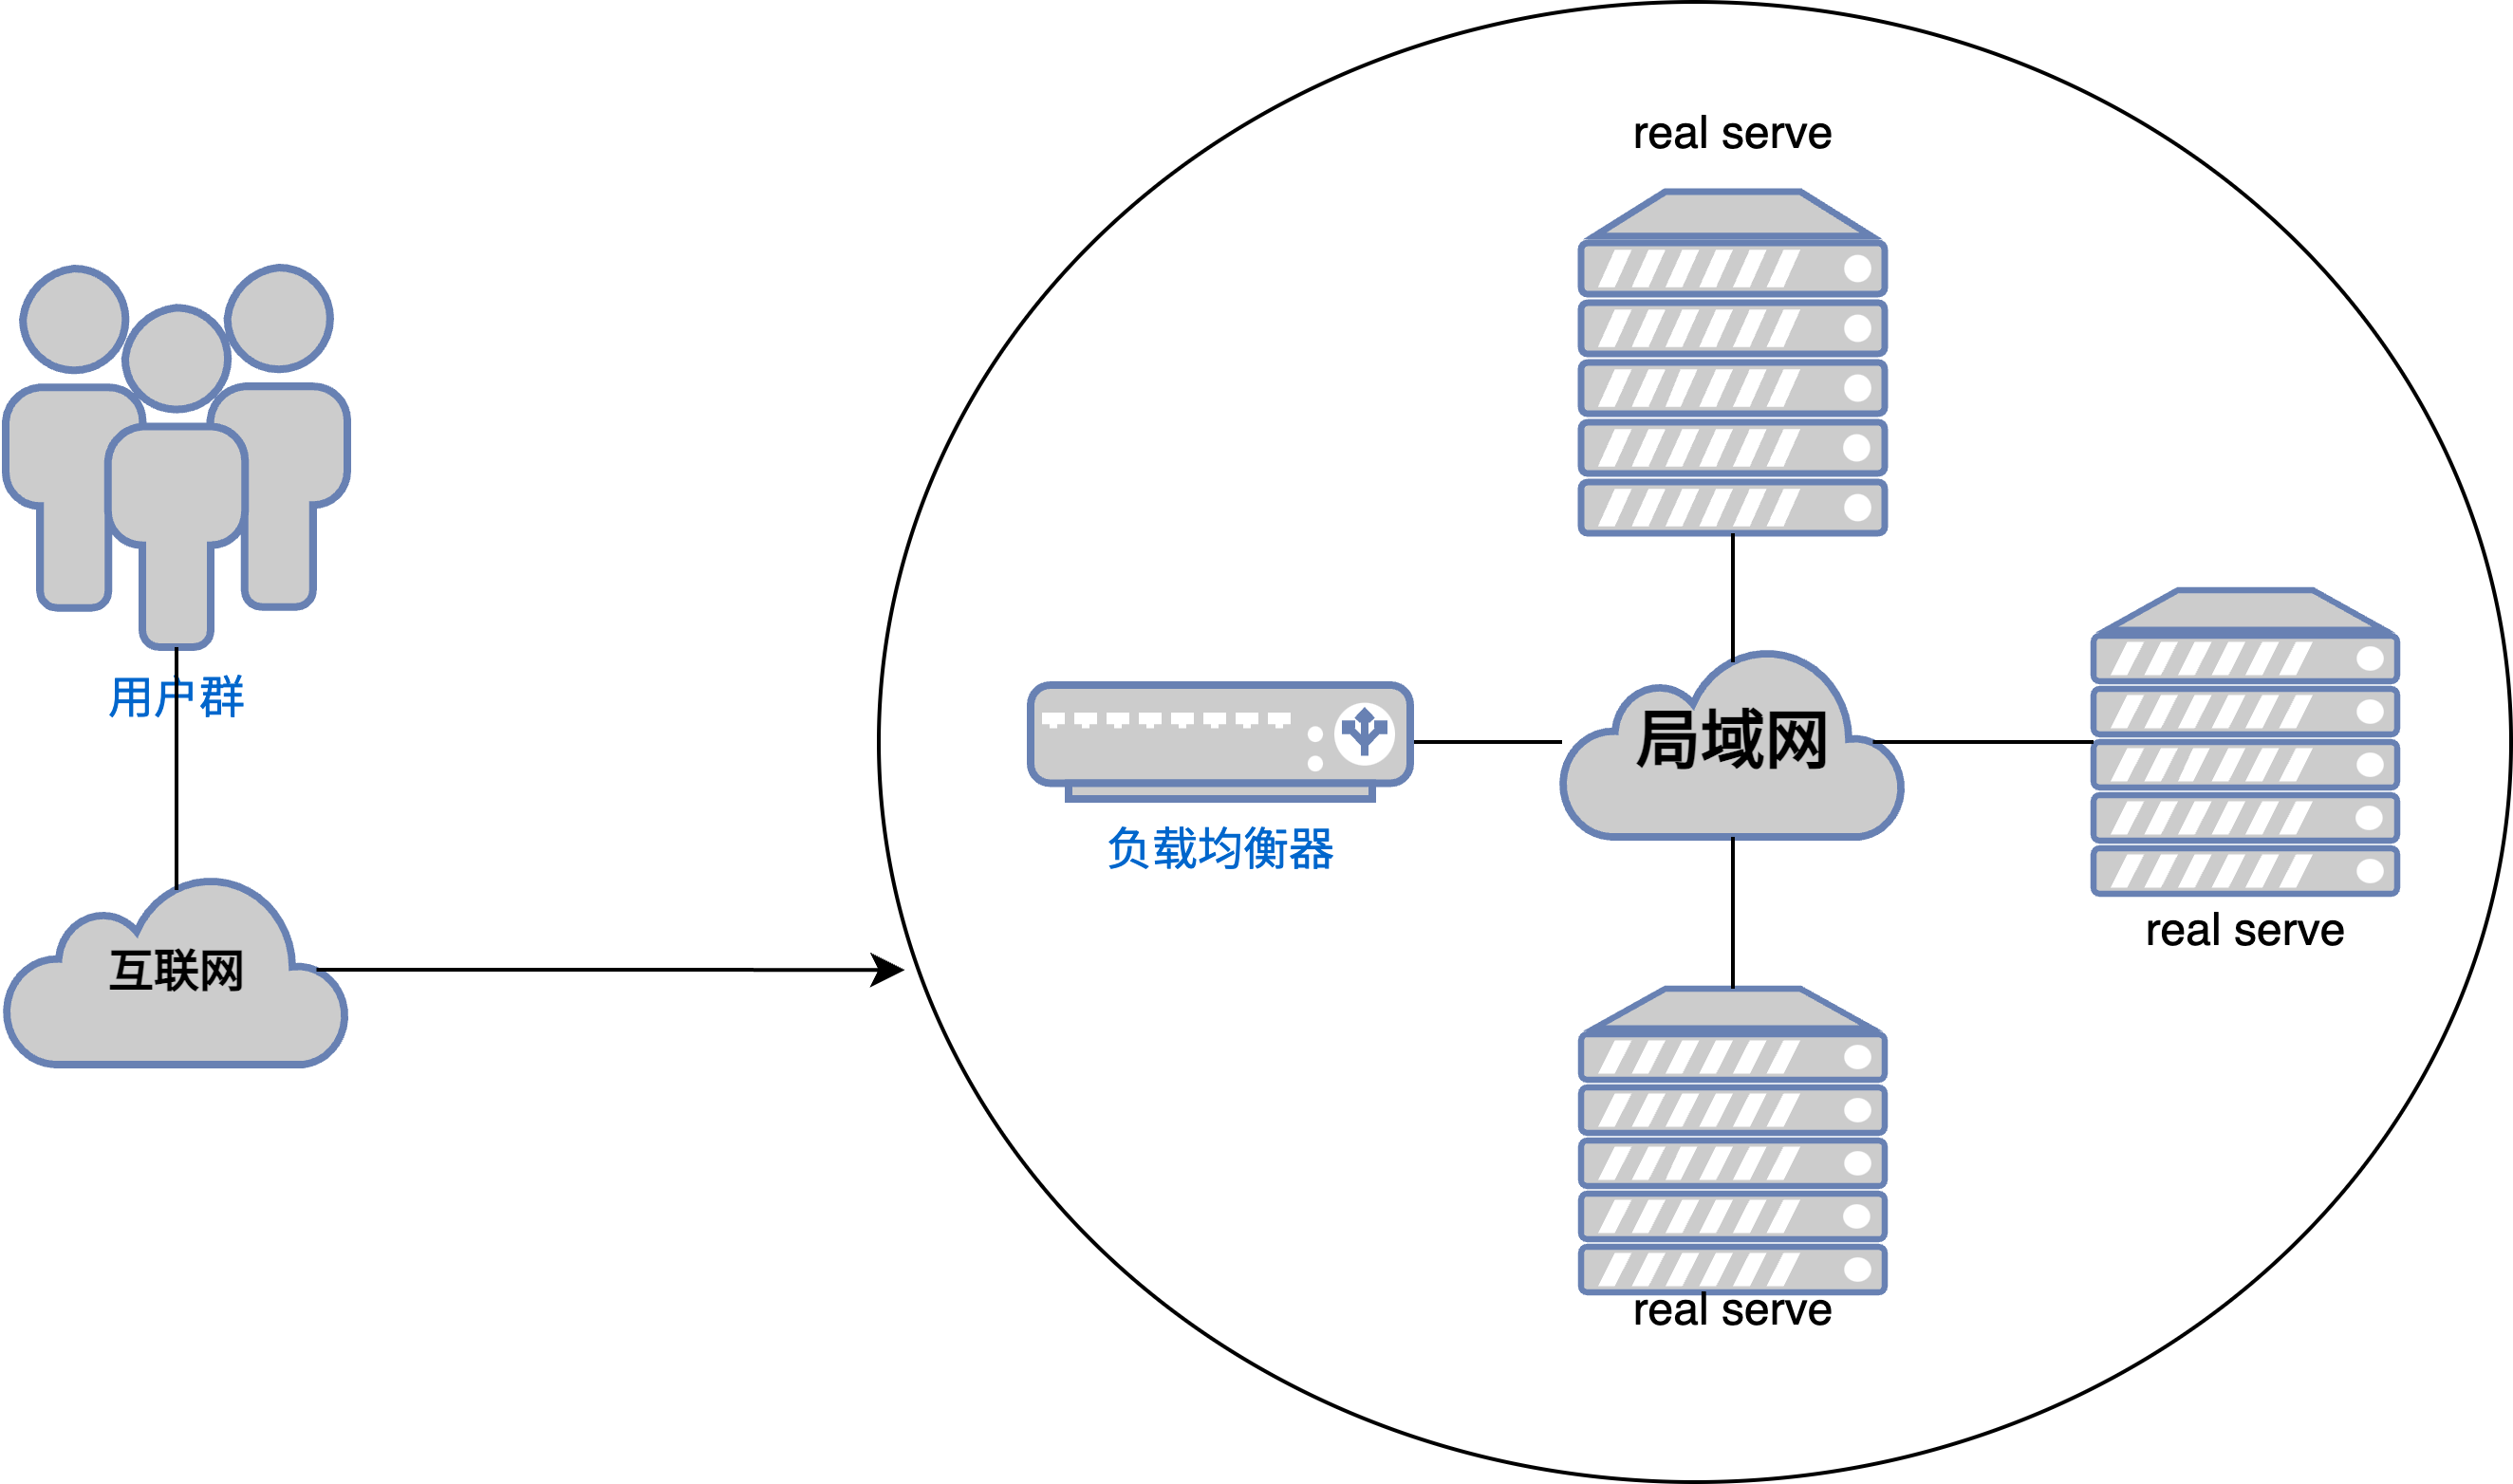
\includegraphics[width=\textwidth]{figures/负载均衡集群基本结构.png}
	\caption{负载均衡集群的基本架构}
\end{figure}

尽管负载均衡集群技术大幅提高了服务器处理请求的能力,但其仍面临一些不可忽视的限制。
具体而言,负载均衡器缺乏实时监测集群服务器性能状态的能力,这一不足可能在请求分配时引起服务器过载或闲置的问题。
为克服这一障碍,负载均衡集群系统往往在分发请求的服务器上实施性能监控程序,旨在动态追踪业务服务器的负载情况。
借助此类监控手段,能够实时获取上游服务器的负载动态,进而精细化请求分配机制。
本文旨在探索在负载均衡集群环境中,时间序列学习预测算法的应用及其优化策略,并以此为研究重点。

\subsection{服务器性能指标}

负载均衡集群通过性能监控程序密切跟踪上游服务器的运行状态,核心策略在于如何挑选出既易于获取又占用较少系统资源且能精准反映服务器资源利用状况的负载指标,这一系列指标被统称为负载向量。
研究显示,衡量服务器性能的指标一般会综合考量如下几个维度:CPU占用率、内存使用量、网络带宽及磁盘I/O情况。通过研究亦可见,采纳不同的性能评价指标会对负载均衡算法的效果产生显著影响。并且,这些评价指标随着应用环境的变化而相应调整。

通过监控资源利用率(如 CPU、内存、磁盘 I/O 和网络带宽),系统可以确保工作负载均匀分布在所有可用资源上。
这样可以确保没有任何单个资源的过度使用,从而最大化整体性能。当业务增长时,可以根据资源利用率数据来决定何时需要
扩展硬件或调整系统配置,以优化性能和成本。

CPU是计算机架构中至关重要的硬件组件,其利用效率在很大程度上决定了服务器节点的性能表现。一旦CPU的使用率超过了合理范围,就会导致性能降低和负载增加,从而影响服务器的整体运行效率。CPU的性能不仅受到核心数和运行频率的影响,而且由于不同CPU型号间存在差异,因此在将CPU性能纳入评估服务器负载的向量时显得尤为复杂。

此外,服务器节点的内存访问速度显著影响CPU处理任务的效率。随着网络请求的逐渐增加,相应地,
数据访问需求也会增加,进而导致内存中数据请求和传输活动变得更加频繁。
这种情况可能会引起更多的分页错误或缺页现象,不仅严重降低了CPU的处理效率,还削弱了服务器节点处理请求的能力,
最终对整个服务器集群的性能水平产生不利影响。

如果对服务器的高性能计算需求较大,那么CPU使用率和内存利用度应优先作为主要的评价指标,反之,如果所处理的任务需要频繁进行数据传输和存储,那么网络带宽和磁盘I/O则更能反映出这种任务类型的性能状况。

以上提到的负载向量指标只能表示服务器节点的实时工作状态\cite{mahato2017scheduling},而队列长度则更能反映出处理请求任务的完整流程,这是一个更具预测性的评价方法。当任务入队列时,如果服务器负载过高,将无法接受更多的任务。性能监控程序可以监控到服务器的实时性能,但对于网络任务来说,它们是按队列被负载均衡器分发的。虽然我们可以测量队列长度,但无法知道队列中的任务消耗资源的具体情况,所以队列长度并不能完全反映出节点的负载能力。我们通常会关注CPU的队列长度,以此获得更全面的评价。

获取CPU队列长度的方法有两种,一种是计算一段时间内的平均队列长度,另一种是获取某个特定时刻的队列长度。这两种方式可共同用来营造出服务器节点负载的全景视角。

考虑到CPU性能和任务队列长度单独来看无法全面评估服务器的负载状况,我们需要构建一个融合多种不同指标的综合负载评价体系。
通过数学计算,我们可以得到一个能够全面反映节点负载程度的新指标。根据黄伟华的研究,在“一种特征加权模糊聚类的负载均衡算法”\cite{黄伟华2017一种特征加权模糊聚类的负载均衡算法}中,主要提出了三种方法。
首先,一种方法是以队列长度为主要考量因素,而将CPU和磁盘I/O作为辅助指标参与评价,这能够提供关于任务处理能力的初步信息。
其次,另一种方法是将队列长度和资源利用率(如CPU和内存使用情况)结合在一起,作为一个整体的评价指标,从而更加全面地反映服务器的当前状态。
最后,采用优先级方式,即首先考虑影响最大的指标,如内存占用情况,然后在内存资源充足的条件下,再综合考虑其他辅助指标。这些方法展现了如何从不同角度和层面对服务器的负载状况进行更准确的评估,以便实施更有效的负载均衡策略。

\subsection{本文选择的参考指标}

依据自身经济和技术情况,选择使用观察节点的各种资源利用情况作为负载均衡能力的指标,并选取了 CPU,内存,磁盘 I/O 和网络带宽作为评价各个节点性能的指标。
具体的系统状态评价对应的资源利用率情况本文进行了整理,如下图表所示。

\noindent\begin{longtblr}[caption={稳定系统的资源状态和评价}]
	{hlines,vlines, colspec = {X[c]X[c]X[c]}}
	性能指标                     & 资源利用率          & 状态评价 \\
	\SetCell[r=3]{c} CPU 利用率 & 70\%           & 好    \\
	                         & 85\%           & 坏    \\
	                         & 90\%+          & 很差   \\
	\SetCell[r=3]{c} 磁盘IO    & <30\%          & 好    \\
	                         & <40\%          & 坏    \\
	                         & <50\%          & 很差   \\
	运行队列                     & <2*CPU数量       & 好    \\
	网络带宽                     & <30\%带宽        & 好    \\
	\SetCell[r=3]{c} 内存      & 没有页交换          & 好    \\
	                         & 每个 CPU每秒10个页交换 & 坏    \\
	                         & 更多的页交换         & 很差   \\
\end{longtblr}

在处理大规模任务和网络请求时,服务器集群可能遭遇负载不均衡现象,表现为某些节点过载而其他节点则处于低负载状态。
这种情况下,必须对集群内各节点的负载情况实施实时监控,并据此调整任务分配,以提升集群整体性能。

为准确评估服务器节点的当前负载水平,可以采用特定的数学模型进行计算。该模型将综合考虑多种负载指标,
包括CPU、内存、磁盘和网络带宽的使用情况。例如,设定 $L_{j}$ 为第j个节点的负载指标,
函数 $f()$ 则为一种整合上述性能指标的函数,可能采取加权和或其他类型的聚合形式。
例如:$L_{j} = f(C_{j}, M_{j}, D_{j}, N_{j})$,确保精确反映各节点的负载状态。
\[
	X = W_{cpu} \cdot C_j + W_{mem} \cdot M_j + W_{io} \cdot D_j + W_{net} \cdot N_j\tag{1.1}
\]
$X$ 为当前服务器节点的总体剩余性能。通过对 $X$ 值的监控,观察和比较其变化范围作为判断负载均衡器是否需要修改请求任务分配方案的根据。

\section{负载均衡技术}

\subsection{什么是负载均衡}

负载均衡是在支持应用程序的资源池中平均分配网络流量的一种方法。现代应用程序必须同时处理数百万用户,并以快速、可靠的方式将正确的文本、视频、图像和其他数据返回给每个用户。为了处理如此高的流量,大多数应用程序都有许多资源服务器,它们之间包含很多重复数据。负载均衡器是位于用户与服务器组之间的设备,充当不可见的协调者,确保均等使用所有资源服务器。

\subsection{负载均衡的优势}

负载均衡可以定向和控制应用程序服务器与其访客或客户端之间的互联网流量。因此,它可提高应用程序的可用性、可扩展性、安全性和性能。

(1)应用程序可用性

服务器故障或维护可能会增加应用程序停机时间,使访客无法访问应用程序。
负载均衡器可以通过以下方式提高系统的容错能力,自动检测服务器问题并将客户端流量重定向到可用服务器。
运行应用程序服务器维护或升级而无需使应用程序停机,为备份站点提供自动灾难恢复,
执行运行状况检查并防止出现可能导致停机的问题。

(2)应用程序可扩展性

可以使用负载均衡器在多个服务器之间智能地定向网络流量。
应用程序可以处理数千个客户端请求,防止任何一台服务器出现流量瓶颈,
预测应用程序流量,以便可以在需要时添加或移除不同服务器,
为系统增加冗余度,使我们可以放心扩展。

(3)应用程序安全

负载均衡器具有多项内置的安全功能,它们是应对分布式拒绝服务攻击的有用工具,
在这种攻击中,攻击者会用数百万个并发请求淹没应用程序服务器,从而导致服务器故障。负载均衡能够做到:
监控流量并阻止恶意内容,预测应用程序流量,
将攻击流量自动重定向到多个后端服务器,以最大限度减少影响,
通过一组网络防火墙路由流量,以提高安全性。

(4)应用程序性能

负载均衡器通过增加响应时间和减少网络延迟来提高应用程序性能。它们可以执行诸如以下几项关键任务:
在服务器之间平均分配负载以提高应用程序性能,将客户端请求重定向到地理位置较近的服务器以减少延迟;
确保物理和虚拟计算资源的可靠性和性能。

\subsection{负载均衡的类型}

实现负载均衡的方式有很多种,最常见的时间负载均衡类型有三种。

(1)软件和硬件负载均衡

基于硬件的负载均衡器是一种硬件设备,可以安全地处理千兆字节的流量并将其重定向到数百个不同的服务器。可以将其存储在数据中心,并使用虚拟化创建多个可以集中管理的数字或虚拟负载均衡器。
基于软件的负载均衡器是执行所有负载均衡功能的应用程序。可以将它们安装在任何服务器上,也可作为完全托管的第三方服务的形式访问。

硬件负载均衡器需要初始投资、配置和持续维护。也可能不会满负荷使用它们,尤其只是为了处理高峰时段的流量高峰。如果流量突然增加到超出其当前容量,这会影响整体服务器集群的稳定性和可靠度,直接的影响用户,
直到企业能够购买到,并配置好整体的服务器集群,以便于应付下一次突然的流量高峰。
相比之下,基于软件的负载均衡器要灵活得多\cite{常智2013高性能}。
它们可以轻松地纵向扩展或缩减,并且与现代云计算环境更加兼容。随着时间推移,它们的设置、管理和使用成本也会降低。

(2)静态和动态负载均衡

静态负载均衡是一种基于预设规则的负载分配策略,常见的方法包括加权轮询和IP-HASH等。然而,该策略在请求分发过程中并未考虑服务器的实时负载性能,这可能导致性能优越的服务器过载,而性能一般的服务器却处于轻载甚至空闲状态。这种情况会导致集群资源利用率低下,系统性能大打折扣。
尽管静态负载均衡具有易于实现、配置简便等优点,因而得到了广泛应用,但其固有缺陷不容忽视,亟需引起关注。

动态负载均衡依赖于更为复杂的技术支持。它在静态负载均衡策略的基础上进一步考虑了集群中各服务器的实时运行状态,
通过监测服务器实时负载的指标变化来动态地调整请求的分发比例。这种方法旨在最大化地利用集群资源来处理大量并发请求,
实现真正意义上的负载动态平衡。尽管动态负载均衡需要一定的系统资源开销,实践证明它能够显著提高集群的整体性能。
对资源较为有限的小型企业来说,实施动态负载均衡可能存在一定的挑战,但对大型企业而言,这些额外的成本通常是可接受的。
关于负载均衡技术的不同类型,下面将分析使用Nginx作为负载均衡器时的几种常见策略。

\begin{longtblr}[
	caption = {常见Nginx负载均衡算法分析表},
	]{
	width = \linewidth,
	colspec = {Q[171]Q[152]Q[294]Q[321]},
	cell{2}{1} = {r=3}{},
	cell{5}{1} = {r=3}{},
	vlines,
	hline{1,8} = {-}{0.08em},
	hline{2,5} = {-}{},
	hline{3-4,6-7} = {2-4}{},
		}
	负载均衡算法分类 & 算法名     & 优点              & 缺点                 \\
	负载均衡算法分类 & 轮询算法    & 配置简单            & 不能考虑后端服务器性能差异      \\
	         & 加权轮询算法  & 能够考虑不同服务器的性能差异  & 不能考虑负载后服务器的状态变~化   \\
	         & IP 哈希法  & 可以解决~session~问题 & 但在~Nginx~非最前服务器后失效 \\
	动态负载均衡   & 加权最小连接法 & 考虑处理能力的不同       & 无法衡量服务器负载状态        \\
	         & 最短响应时间法 & 根据服务器响应时间分配请求   & 通信开销过大             \\
	         & 基于资源的方法 & 性能最大化,控制分散灵活    & 配置复杂,不一~定反映实际负载
\end{longtblr}

(3)四层到七层负载均衡

大型的网站服务一般会用这样的架构,在业务应用前面加七层负载均衡,然后在七层负载均衡前面加四层负载均衡。当用户发送 HTTP 请求的时候,请求会(经过机房内的路由器,交换机等设备)首先到达四层负载均衡,四层转发给七层,七层转发给应用。
四层负载均衡只解析网络包到第四层,根据四层的内容(比如 TCP port,IP 等)就能确定转发给谁,
七层负载均衡解析网络包到第七层,要根据七层的内容(比如 HTTP URL path,HTTP header 等)才能确定转发给谁。

七层即应用层\cite{pak2015efficient},要解析 HTTP 内容(不仅仅是 HTTP,其他应用层协议的负载均衡,比如一些数据库 proxy,gRPC 代理,等等,
都需要解析完成应用层才能确定转发目标),首先要将 Header 全部读完,读完之后要看下
Content Length 是有多长,然后知道 Body 要读到哪里。根据不同的 URL Path,
还要确定路由到哪一个 upstream。

在传输层级,也就是我们常说的四层,负载均衡器主要关注用户任务的处理。首先,根据预先配置的负载均衡策略,负载均衡器会在内部网络中挑选出最适合的服务器。
然后,它将请求报文中的目标IP地址和端口号修改为选中的服务器的IP地址和端口号,接着建立TCP链接并转发请求。最后,它会将服务器的响应结果返回给用户。Nginx可模拟这一过程,如下图\ref{four_land_balance}所示。

\begin{figure}[htb]
	\centering
	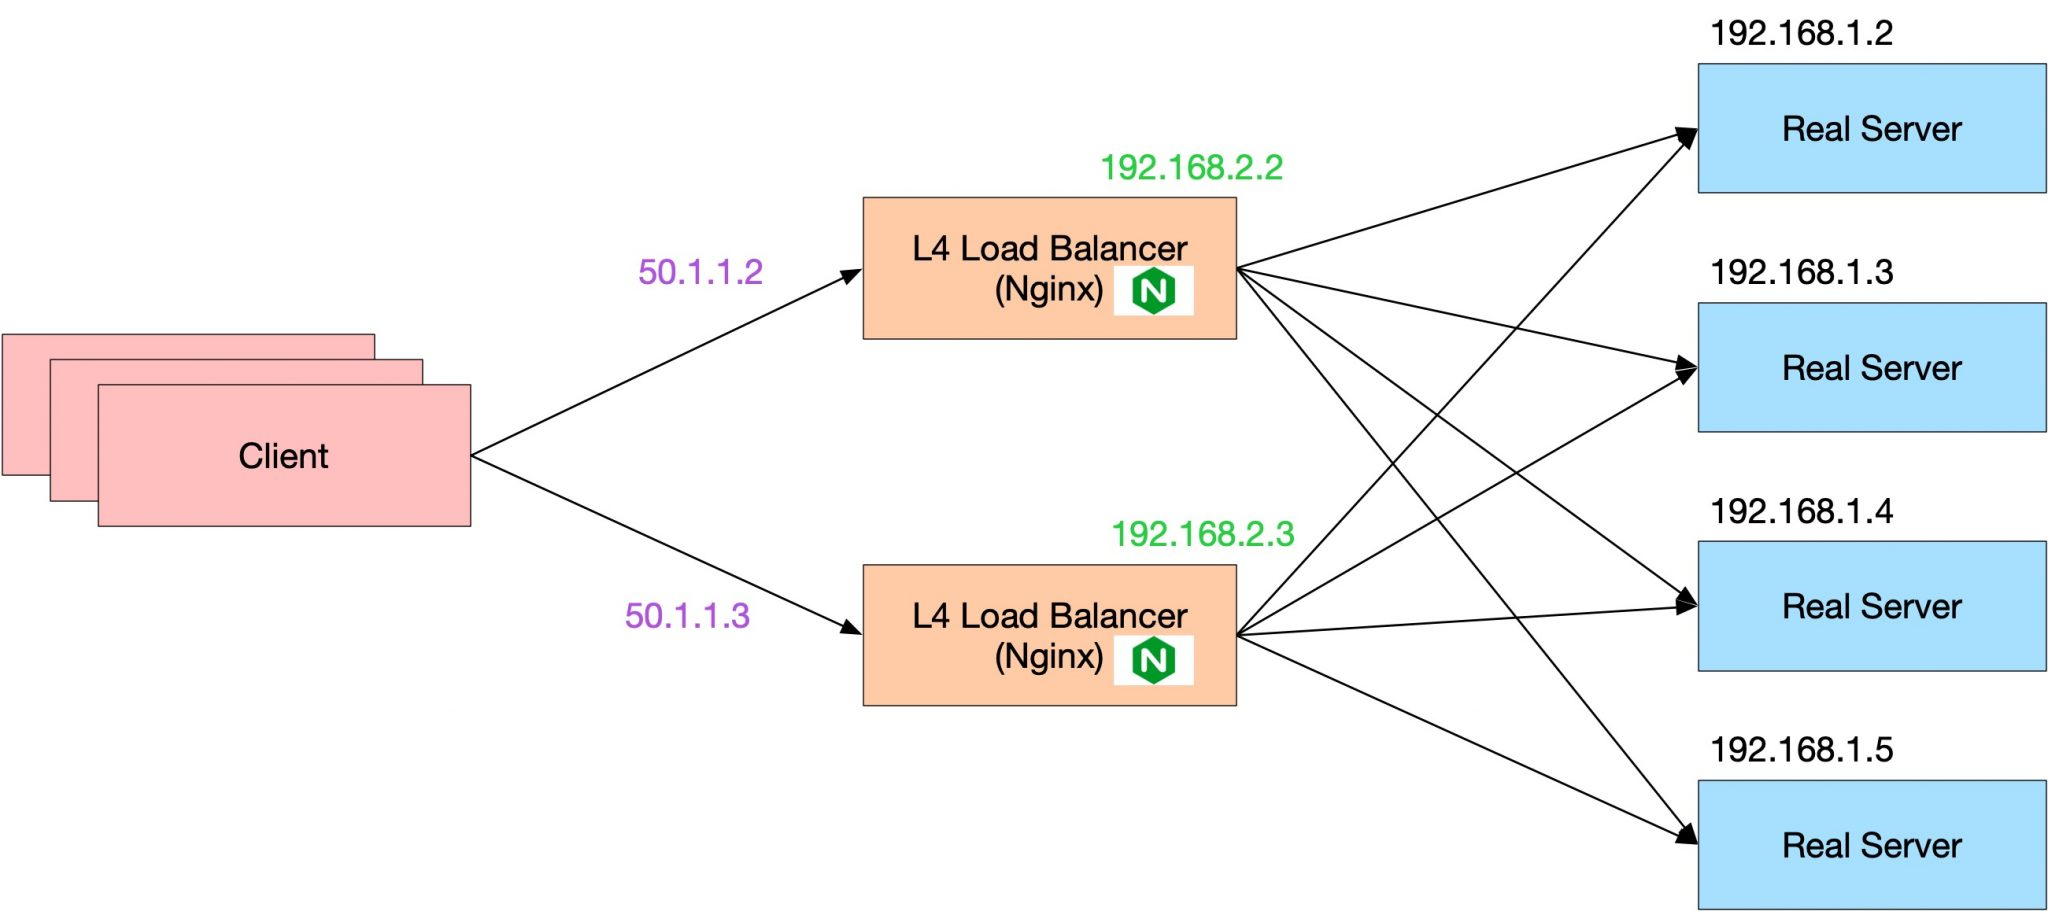
\includegraphics[width=\textwidth]{figures/nginx-l4lb-2048x911.jpg}
	\caption{Nginx 作为四层负载均衡使用}
	\label{four_land_balance}
\end{figure}

\section{Nginx 服务器}

Nginx以其轻量化、内存消耗低和高并发处理能力强等特点,在众多Web服务器中脱颖而出。
它由伊戈尔·赛索耶夫为俄罗斯知名网站Rambler.ru开发,并在2004年10月4日发布了首个公开版本0.1.0。
相对于同期流行的LAMP(Linux Apache MySQL PHP/Python/Perl)堆栈,Nginx通过使用事件驱动的架构,而不是Apache的同步多进程方式,
改善了对任务请求的处理能力,能够在高并发情境下保持资源消耗低、响应速度快且稳定性高\cite{凌质亿2013高并发环境下}。
基于这些优势,包括百度、京东在内的许多大型服务器采用了Nginx。

\subsection{Nginx 工作模式和进程模型}

Nginx 有单进程和多进程两种工作模式,默认进程为多进程。通常情况下,单进程仅仅只在开发环境下调试使用,对外发布服务时
常常使用多进程。多进程模型既是 master-worker 进程模型

\noindent\begin{enumerate}
	\item Nginx 启动后,会产生一个 master 主进程,主进程执行一系列的工作后会产生一个或者多个工作进程 worker
	\item 在客户端请求动态站点的过程中,Nginx 服务器还涉及和后端服务器的通信。Nginx 将接收到的 Web 请求通过代理转发到后端服务器,由后端服务器进行数据处理和组织
	\item Nginx 为了提高对请求的响应效率,降低网络压力,采用了缓存机制,将历史应答数据缓存到本地。保障对缓存文件的快速访问
\end{enumerate}

Nginx的架构设计具有明显的优势:其中的worker进程是并行工作的,彼此之间拥有同等地位。每个worker进程都是通过复制(fork)master进程而生成的。在这一过程中,master进程首先创建了必须监听的socket(即listenfd),接着复制出多个worker进程。这些worker进程共享相同的listenfd,因此新连接建立时,所有worker进程的listenfd都会响应。

为了确保每个新连接仅由一个worker进程处理,Nginx采用了一种竞争机制:在注册读取事件(listenfd)之前,所有worker进程都会尝试获取一个名为accept\_mutex的互斥锁。成功获取互斥锁的worker进程将注册端口的读取事件,并在该事件中调用accept来接受新的连接。

一旦worker进程接受了连接,它就会开始处理整个请求流程:从读取请求开始,对请求进行解析,执行相关处理,产生响应数据,最终发送给客户端,并在完成所有交互后断开连接。这一连串操作构成了Nginx处理请求的完整周期。具体如下图\ref{nginx_multi_process}所示。

\begin{figure}[htbp]
	\centering
	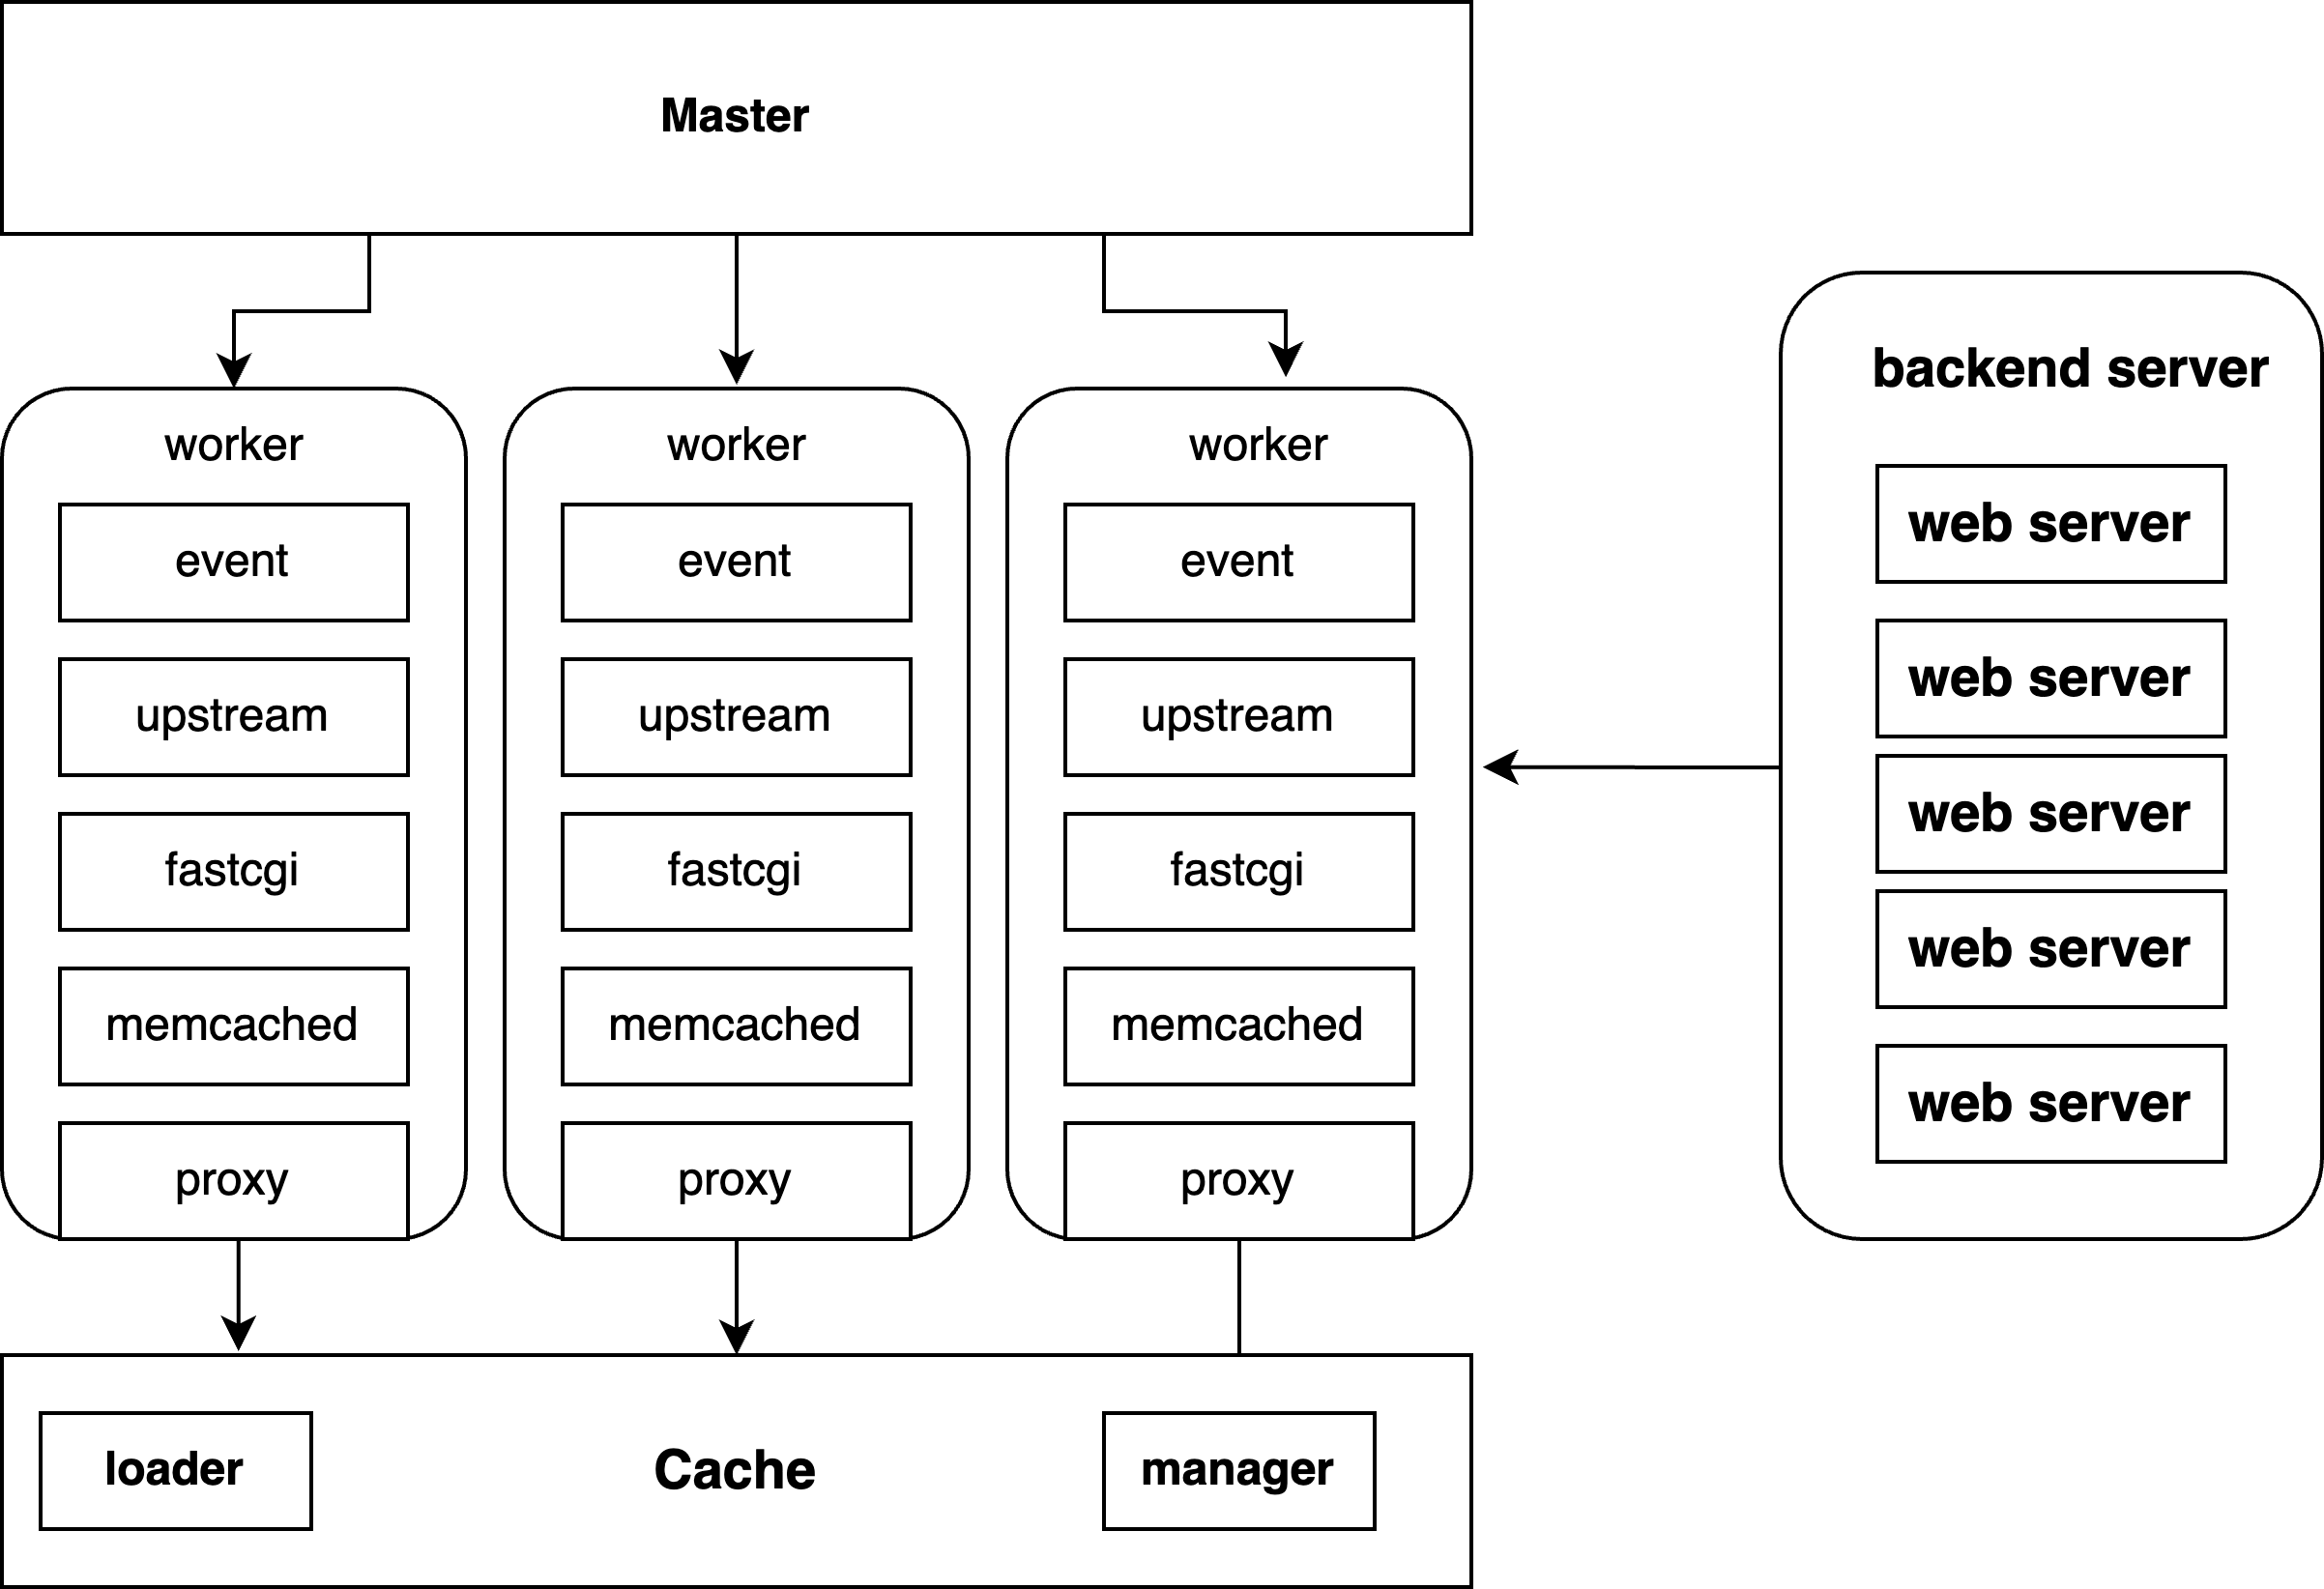
\includegraphics[width=\textwidth]{figures/master-worker.png}
	\caption{Nginx 多进程工作模式}
	\label{nginx_multi_process}
\end{figure}

正是因为Nginx底层采用了eopll(您可能是指epoll)事件驱动模型来实现异步非阻塞IO,这使其能够在极为高效的单进程模型中处理数千甚至数万个并发连接。
每一个worker进程都可以监听并处理多个socket连接,这不仅保障了Nginx卓越的高并发处理能力,并且在这一过程中,它所消耗的内存资源也非常有限\cite{张炜森2018nginx}。
这些特性共同确保了Nginx能够在维护低资源消耗的同时,提供稳定的高性能服务。

\subsection{Nginx的反向代理}

代理,简言之,是一种间接行动的技术手段。当我们希望执行某些操作但不希望直接介入时,就可以借助第三方来完成这些操作。以中介公司为例,当我们需要寻找房源时,我们可以委托中介公司代为搜寻,而不是直接参与房屋寻找的过程。

了解了代理的一般概念后,再来区分正向代理和反向代理。反向代理对于客户端来讲是透明的,客户端无需进行任何特殊配置即可发起请求。
用户的请求首先发送至反向代理服务器,然后由代理服务器选择目标服务器,并从中获取数据。
之后,反向代理服务器会将数据返回给客户端。在这个过程中,反向代理服务器和目标服务器向外界表现为单个实体,这样代理服务器实际上掩盖了真实服务器的IP地址。

理解这两种代理的关键在于代理服务器所代理的对象是什么,正向代理代理的是客户端,我们需要在客户端进行一些代理的设置。而反向代理代理的是服务器,作为客户端的我们是无法感知到服务器的真实存在的。
总结起来就一句话:正向代理代理客户端,反向代理代理服务器\cite{崔娟2023基于Nginx反向代理解决公网上服务跨域问题的研究}。

用一个图片对比正向和反向代理

\begin{figure}[htb]
	\centering
	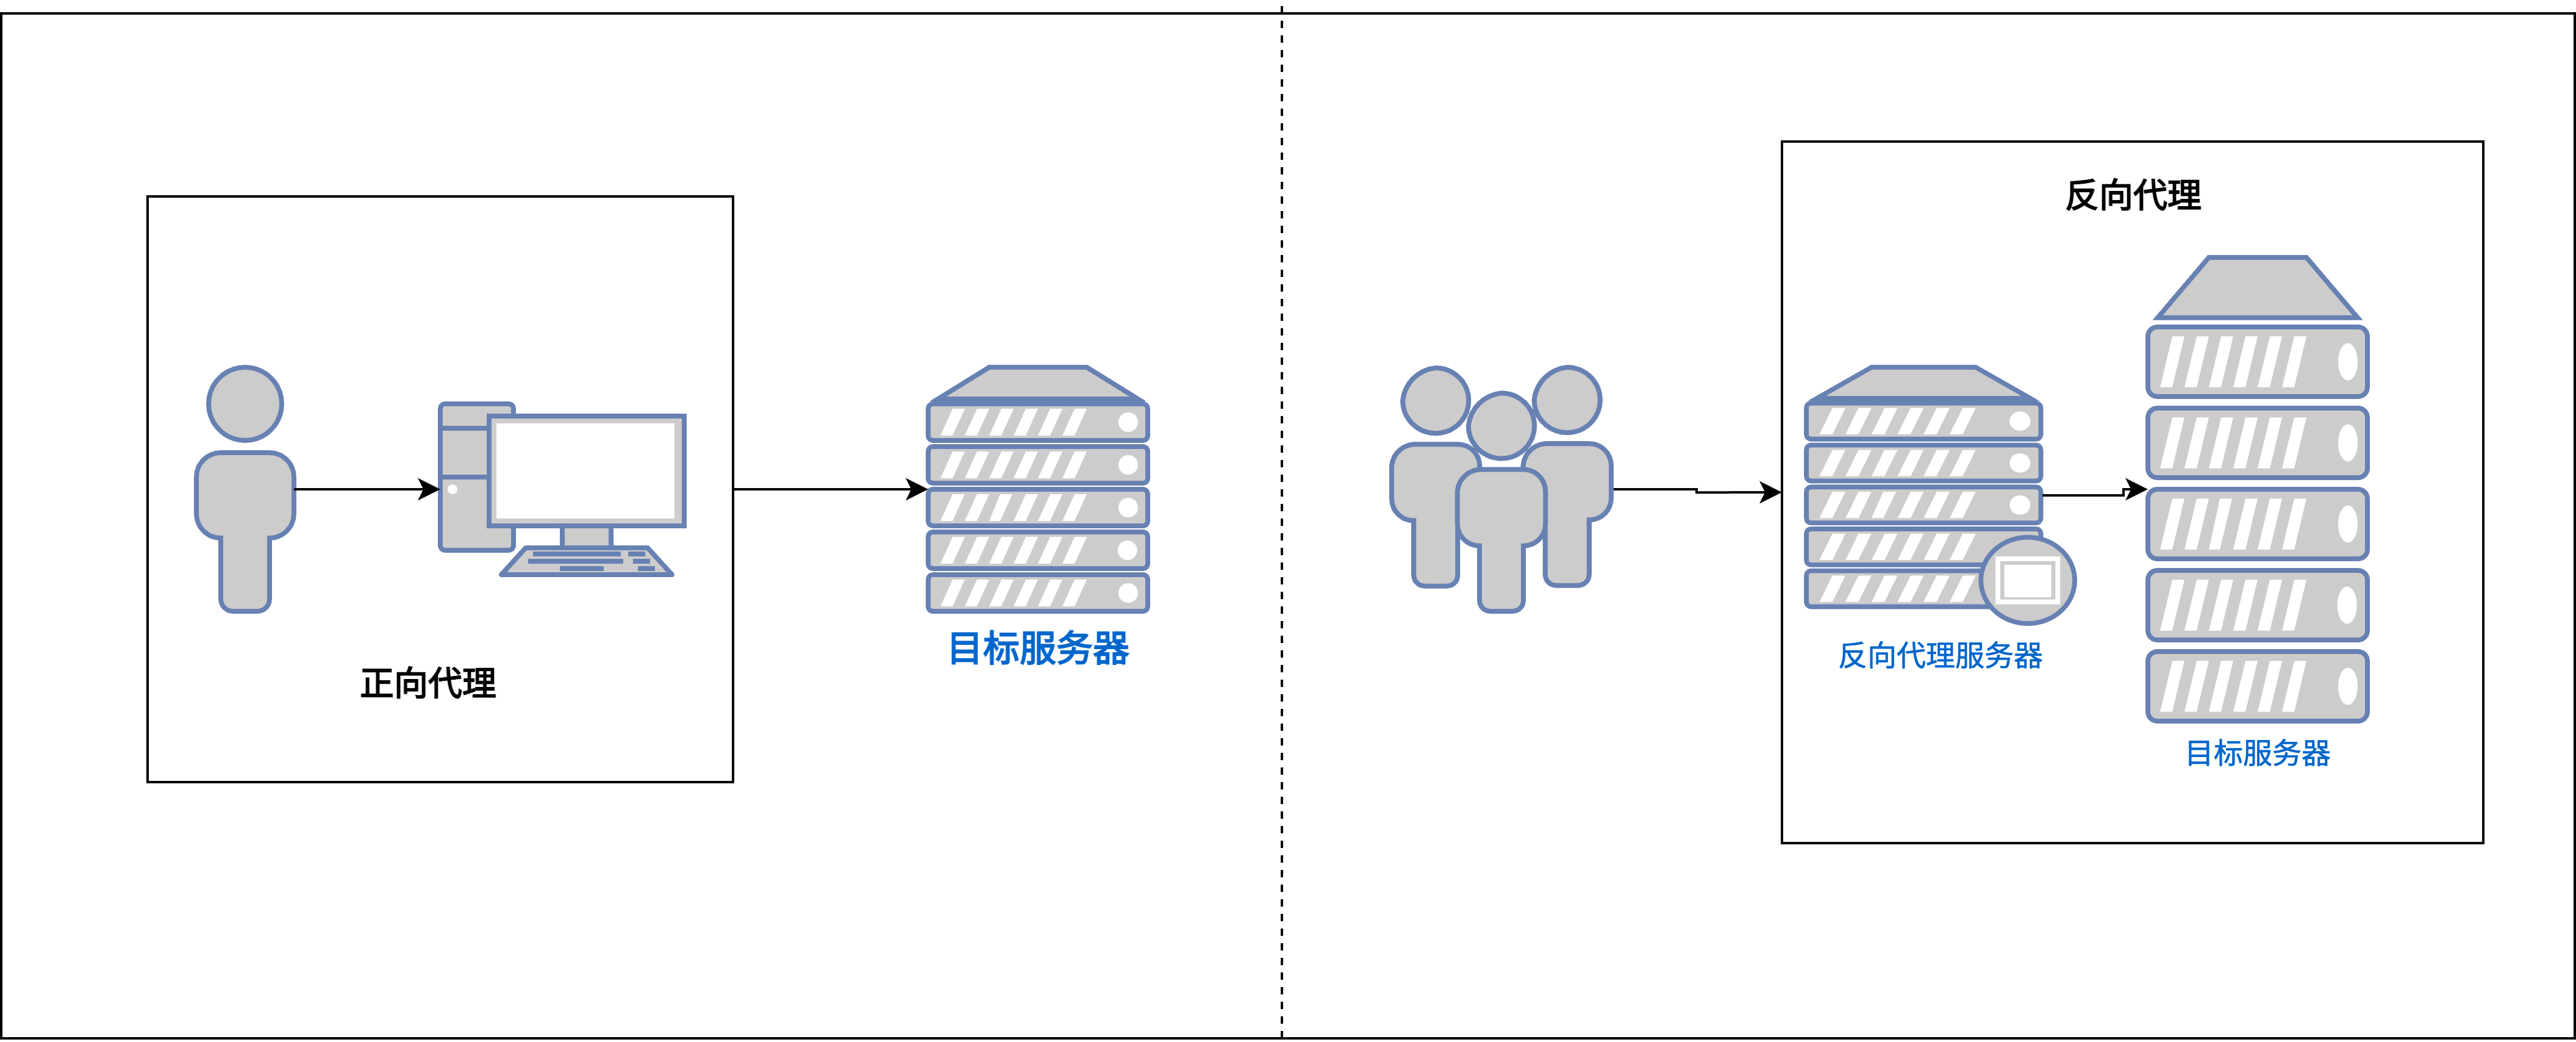
\includegraphics[width=\textwidth]{figures/Forward-Proxy-Reverse-Proxy.png}
	\caption{正向代理与反向代理的对比}
\end{figure}

Nginx的反向代理功能克服了单一服务器的限制,赋予了其在网络上接受、转发及处理数据的强大能力\cite{马原龙2016nginx}。
通过proxy\_pass指令可以轻松设定配置Nginx反向代理,其语法格式为"proxy\_pass URL",其中的URL代表了上游服务器的地址。

Nginx反向代理的一个配置实例如下所示,配置中的“proxy\_set\_headerX-Real-IP”表示定义了一个值为“remote\_addr”的首部“X-Real-IP”,
也即客户端的IP地址。当上游服务器接收到客户端请求时,该自定义的首部将以客户端IP的形式被打印到服务器访问日志中,
这样一来,上游服务器就可以根据真实的客户端IP地址进行日志记录与分析,而不是仅仅依赖于Nginx代理的IP\cite{吴陈2020基于Nginx的服务器集群负载均衡策略的研究与改进}。

\noindent \begin{lstlisting}[caption={Nginx 反向代理默认配置}]
location \index{
  set $upstream_url "";
  proxy_set_header X-Real-IP $remote_addr;
  rewrite_by_lua_file /home/${HOME}/luafile/log.lua
  proxy_pass http://upstream_url;
}
\end{lstlisting}

在客户端与 Nginx 服务器通信的过程中,请求首次到达 Nginx 时,并不会立刻建立与目标(上游)服务器的 TCP 连接来转发该请求。
相反,Nginx 会先将请求缓存在内部的一个队列中,随后按照某种策略与目标服务器建立通信并发送请求。
这种方式有效地平衡了服务器节点间的负载,降低了处理压力。

考虑到客户端和 Nginx 之间通常通过公网进行慢速连接,而 Nginx 和它的上游服务器间则是在更为快速的内部网络中通信,可以利用 HTTP 连接的无状态特性进行一定的优化。
例如,可以在客户端与 Nginx 之间启用 Keep-Alive 功能以保持连接处于活跃状态,并且可选择关闭 Nginx 与上游服务器间的 Keep-Alive 功能,从而释放上游服务器的系统资源,减少负载压力。

当上游服务器处理完客户端的 HTTP 请求并生成相应的响应报文后,这些报文首先会被发送到 Nginx。
在接收过程中,Nginx 会对报文进行必要的处理,比如解析、修改头部信息或者整合多个响应。
完成处理后,Nginx 再将调整后的响应报文发送给客户端。不同于在请求阶段 Nginx 先完全接收再转发,
这一阶段 Nginx 采取的是边接收边转发的模式,大大减少了响应到客户端的时间延迟\cite{邓仲举2012高可靠性集群部署的设计与实现},提高了整体的传输效率。

\subsection{Nginx 负载均衡}

Nginx 自身支持多种负载均衡算法,除了使用源码自带的内置调度算法之外,还可以支持第三方扩展的
负载均衡技术\cite{sufiev2016dynamic}。如果想要开启源码自带的调度算法可以则可以把指定调度算法
的模块打开。一般来说,不需要单独下载某一模块,需要使用时在配置文件中指定即可。Nginx 内置的调度
算法有加权轮询算法、最小连接算法、IP 哈希算法。第三方扩展算法则需要安装第三方模块,将模块放在指定的扩展算法
模块路径,在编译Nginx过程中,扩展算法会一并编译在二进制程序中,最后使用便可以依据配置指令使用指定的
第三方调度算法。常见的第三方调度算法有 fair 响应时间比算法(需要安装ngx\_http\_upstream\_fair\_module),URL 哈希算法(需要安装ngx\_http\_upstream\_hash\_module)
等。下面将对常见的Nginx调度算法进行分析。

(1)加权轮询算法

默认轮询算法(Round Robin)的策略是:将请求“依次”分发到候选机器。如下图\ref{default_bound_balance}所示,轮询负载均衡器收到来自客户端的 6 个请求,编号为 1、4 的请求会被发送到服务端 0;编号为 2、5 的请求会被发送到服务端 1;编号为 3、6 的请求会被发送到服务端 2。

默认的轮询算法是等值轮询,即按照一比一的比例向不同的服务器节点分发请求,当配置文件
没有任何 weight 权值参数是,则采用默认的轮询算法。

\begin{lstlisting}
# 默认的轮询算法
upstream backend {
    server 127.0.0.14:80 max_fails=2 fail_timeout=10s;
    server 127.0.0.15:80 max_fails=2 fail_timeout=10s;
}
\end{lstlisting}

轮询算法,算法的复杂度比较低,执行效率较高,但是不能体现出集群节点内不同的性能差异和负载情况。

\begin{figure}[htbp]
	\centering
	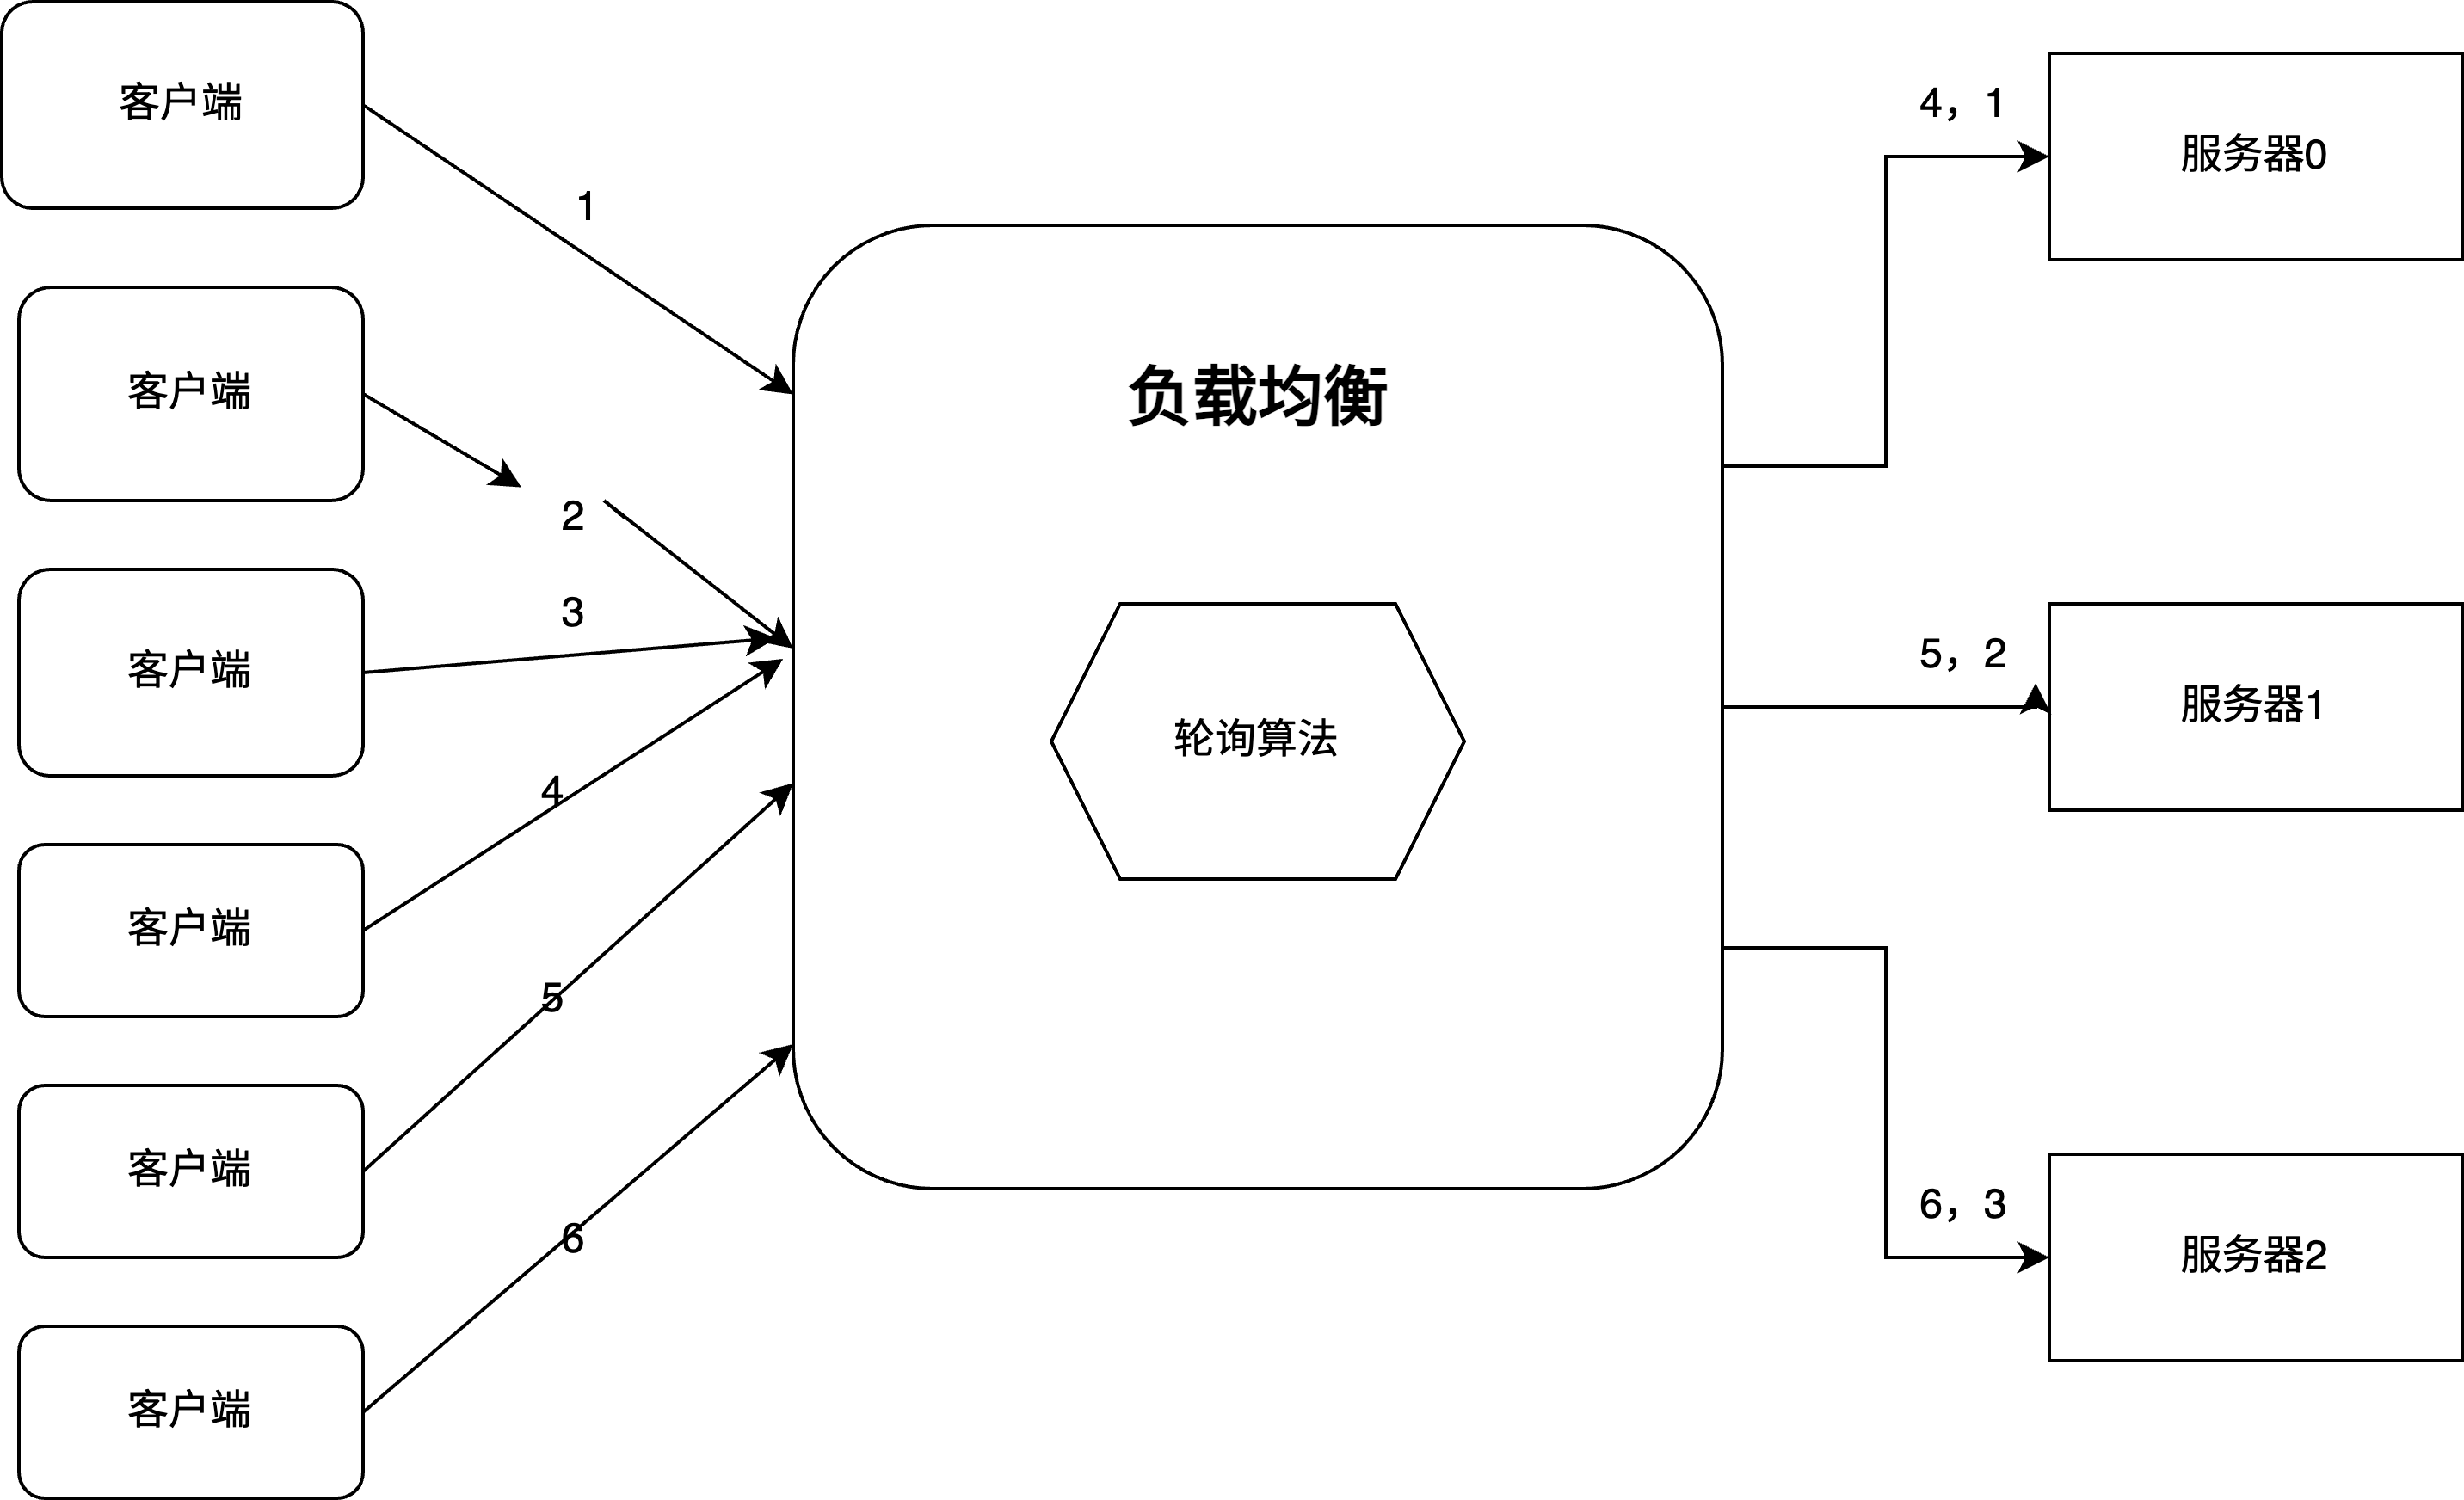
\includegraphics[width=\textwidth]{figures/round-robin.png}
	\caption{默认情况下的负载均衡算法}
	\label{default_bound_balance}
\end{figure}

(2)最小连接算法

最小连接算法(least\_conn)一句话概括就是:按nginx反向代理与后端服务器之间的连接数,
连接数最少的优先分配\cite{周常志2023基于改进加权最小连接数的微服务负载均衡算法研究}。
要根据机器连接数分发,显然要先维护机器的连接数。
因此,最少连接数算法需要实时追踪每个候选机器的活跃连接数;
然后,动态选出连接数最少的机器,优先分发请求。最少连接数算法会记录当前时刻,
每个候选节点正在处理的连接数,然后选择连接数最小的节点。该策略能够动态、
实时地反应机器的当前状况,较为合理地将负责分配均匀,适用于对当前系统负载较为敏感的场景。

\begin{lstlisting}
# 最小连接算法
upstream backend {
    least_conn;
    server 127.0.0.14:80 max_fails=2 fail_timeout=10s;
    server 127.0.0.15:80 max_fails=2 fail_timeout=10s;
}
\end{lstlisting}

最小连接数调度算法通过为每个上游集群节点维护一个计数变量number来跟踪每个节点的连接数。
每当负载均衡器向某个节点分配任务时,相应节点的number值便增加1;当任务完成时,则将该值减去1。Nginx会监控这种计数变量的变化,在每次任务分配时选择当前number值最小的服务器,以此来实现任务的平衡分配。此外,最小连接数算法还能与加权连接算法相结合。通过为性能不同的服务器分配不同的初始权重,算法在分发任务请求时将优先考虑连接数与权重比最小的节点,从而选择出最佳的服务器节点。该算法的流程如图\ref{minlinkconnection}所示。

\begin{figure}[htb]
	\centering
	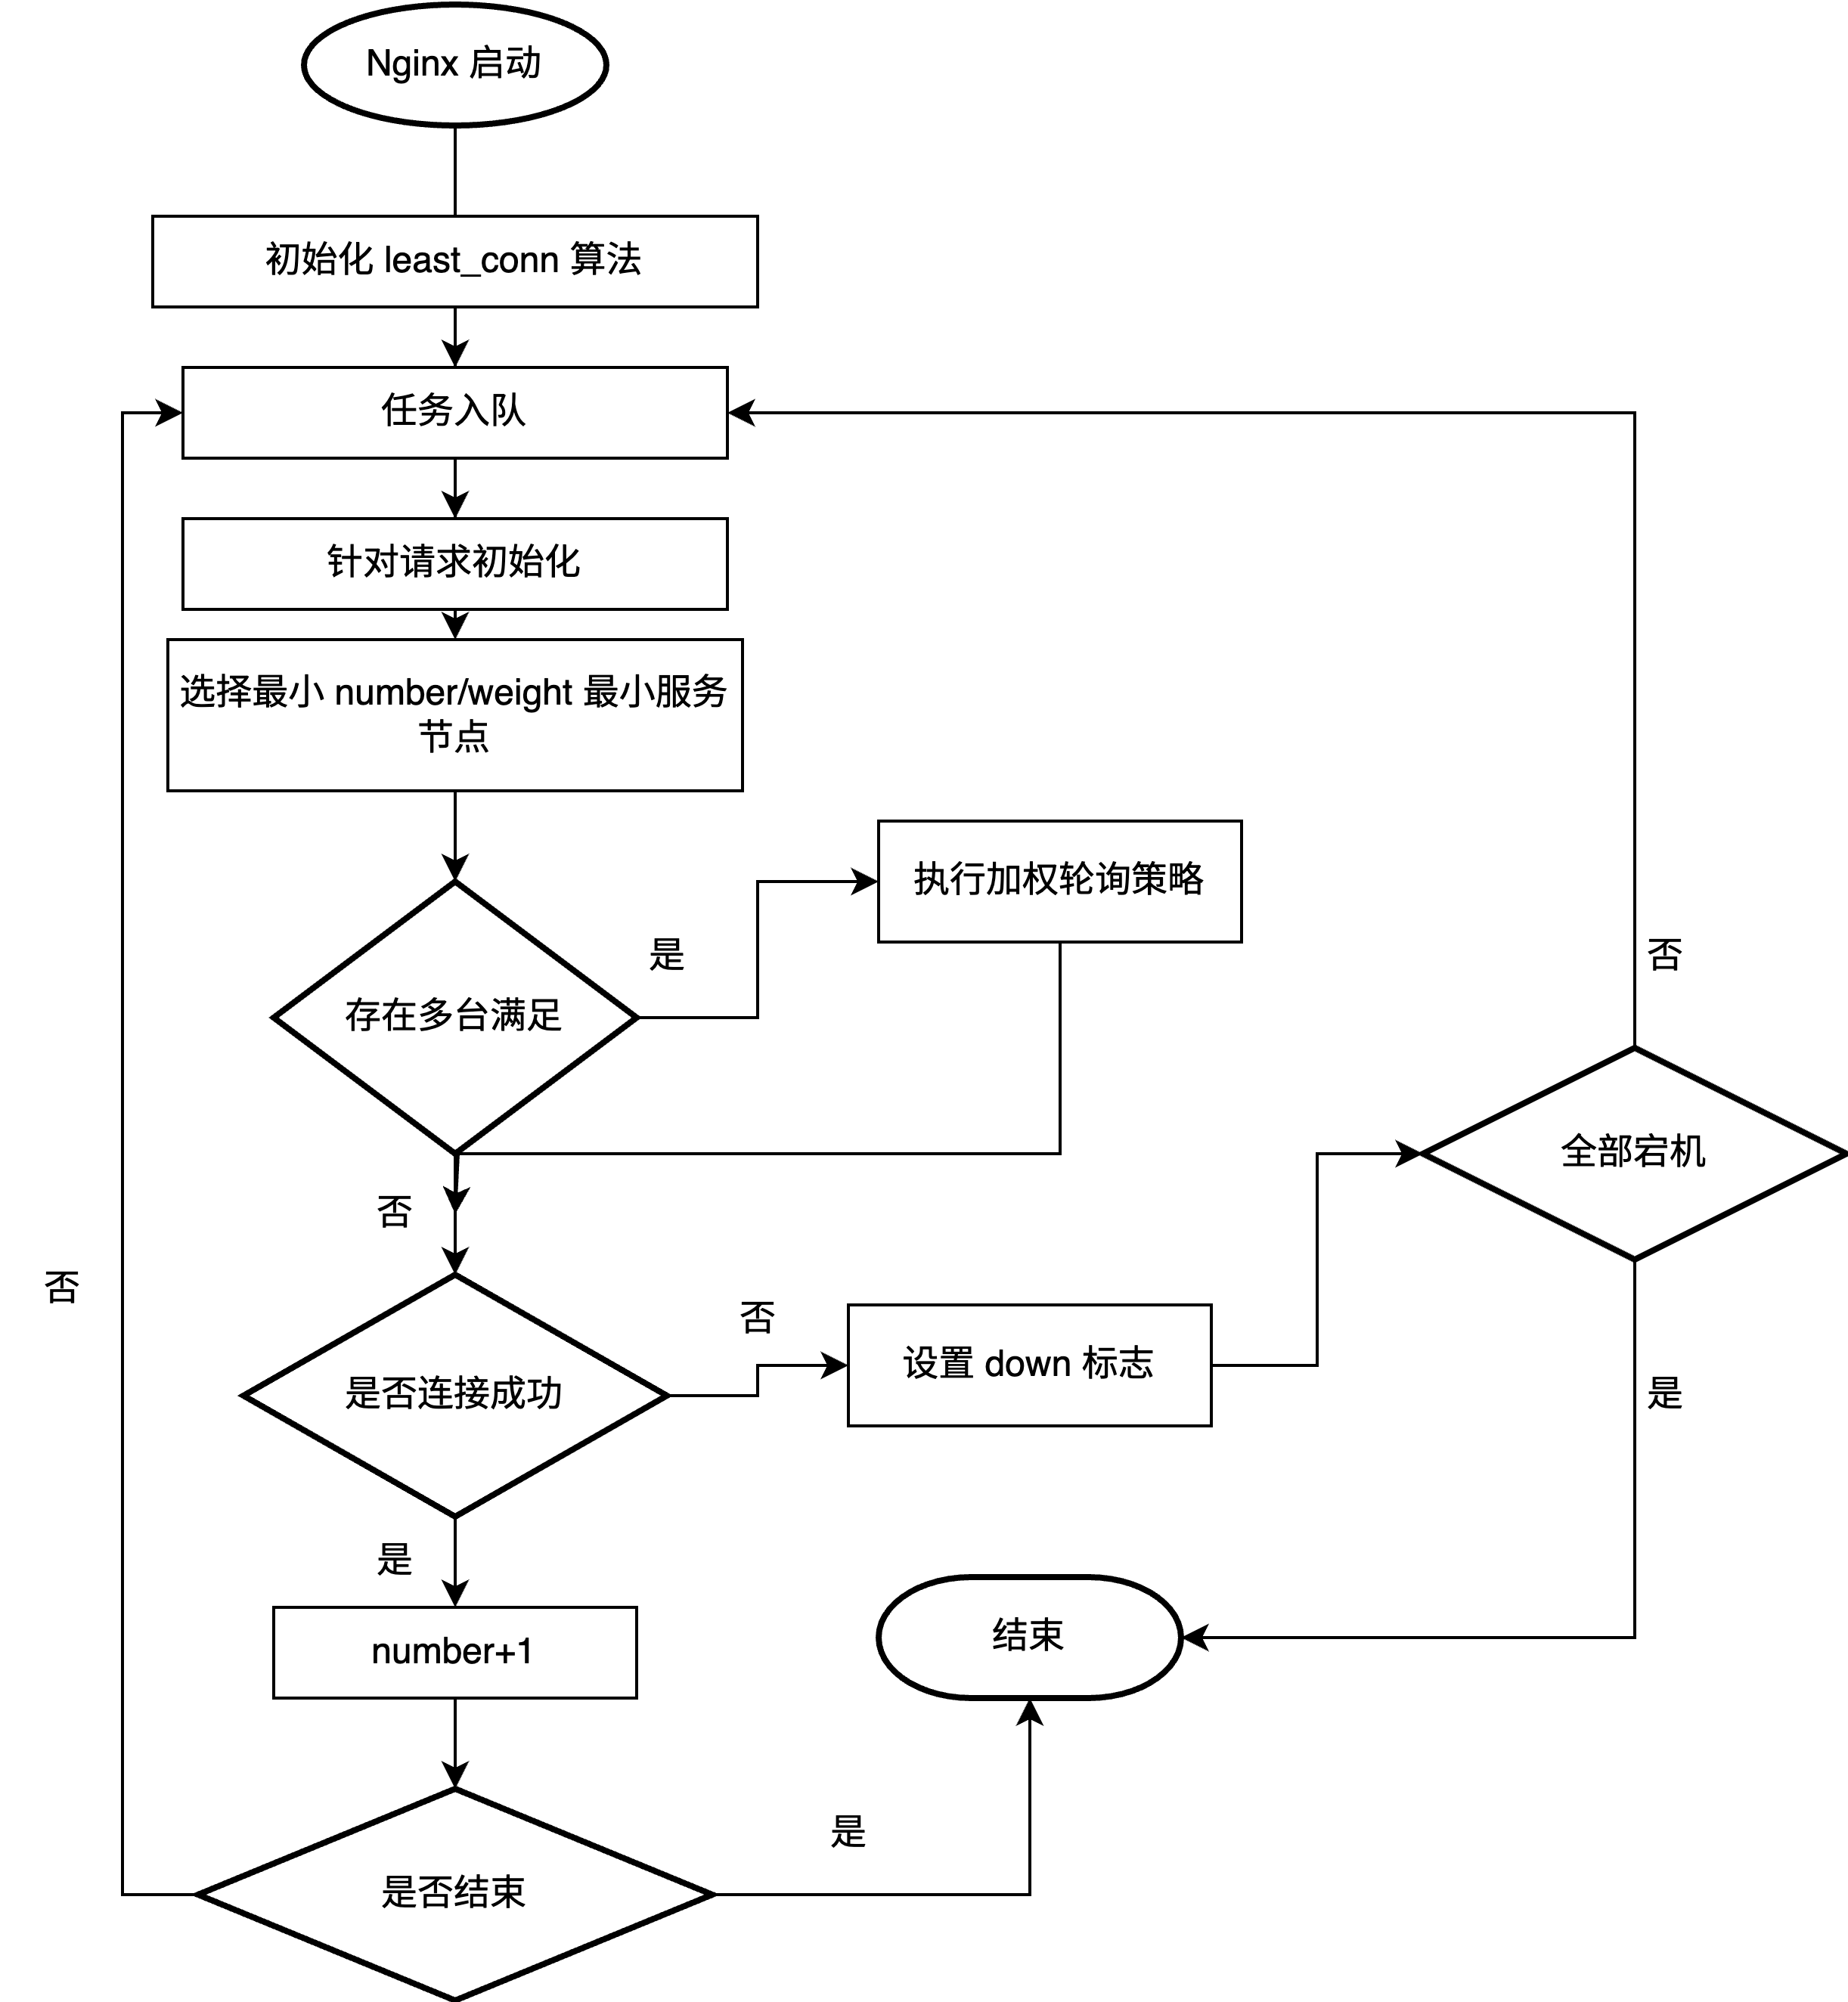
\includegraphics[width=\textwidth]{figures/least-flowchart.png}
	\caption{Nginx 最小连接算法}
	\label{minlinkconnection}
\end{figure}

最小连接数算法考虑了服务器实时负载的动态变化,尝试基于连接数的多少来动态选择用于任务分发的服务器,这在一定程度上克服了加权轮询算法中因请求到达时间间隔不一致而导致的负载不均问题。
然而,由于每个连接上的请求复杂度可能不同,仅凭连接数量来反映服务器的实时负载情况仍存在一定局限性。

(3)IP 哈希算法

哈希算法(Hash)根据一个 key (可以是唯一 ID、IP、URL 等),通过哈希函数计算得到一个数值,用该数值在候选机器列表的进行取模运算,得到的结果便是选中的机器\cite{邱亚飞2021哈希算法的实现与验证}。
哈希算法解决的问题既是人工的判断某个具体任务需要的性能大小,如果该任务消耗的性能较多,负载均衡器将会对该请求连接进行分配到候选的高性能服务器中。
这种算法可以保证,同一关键字(IP 或 URL 等)的请求,始终会被转发到同一台机器上。哈希负载均衡算法常被用于实现会话粘滞(Sticky Session)。
但是 ,哈希算法的问题是:当增减节点时,由于哈希取模函数的基数发生变化,
会影响大部分的映射关系,从而导致之前的数据不可访问。要解决这个问题,
就必须根据新的计算公式迁移数据。显然,如果数据量很大的情况下,迁移成本很高;
并且,在迁移过程中,要保证业务平滑过渡,需要使用数据双写等较为复杂的技术手段。

\begin{figure}[htb]
	\centering
	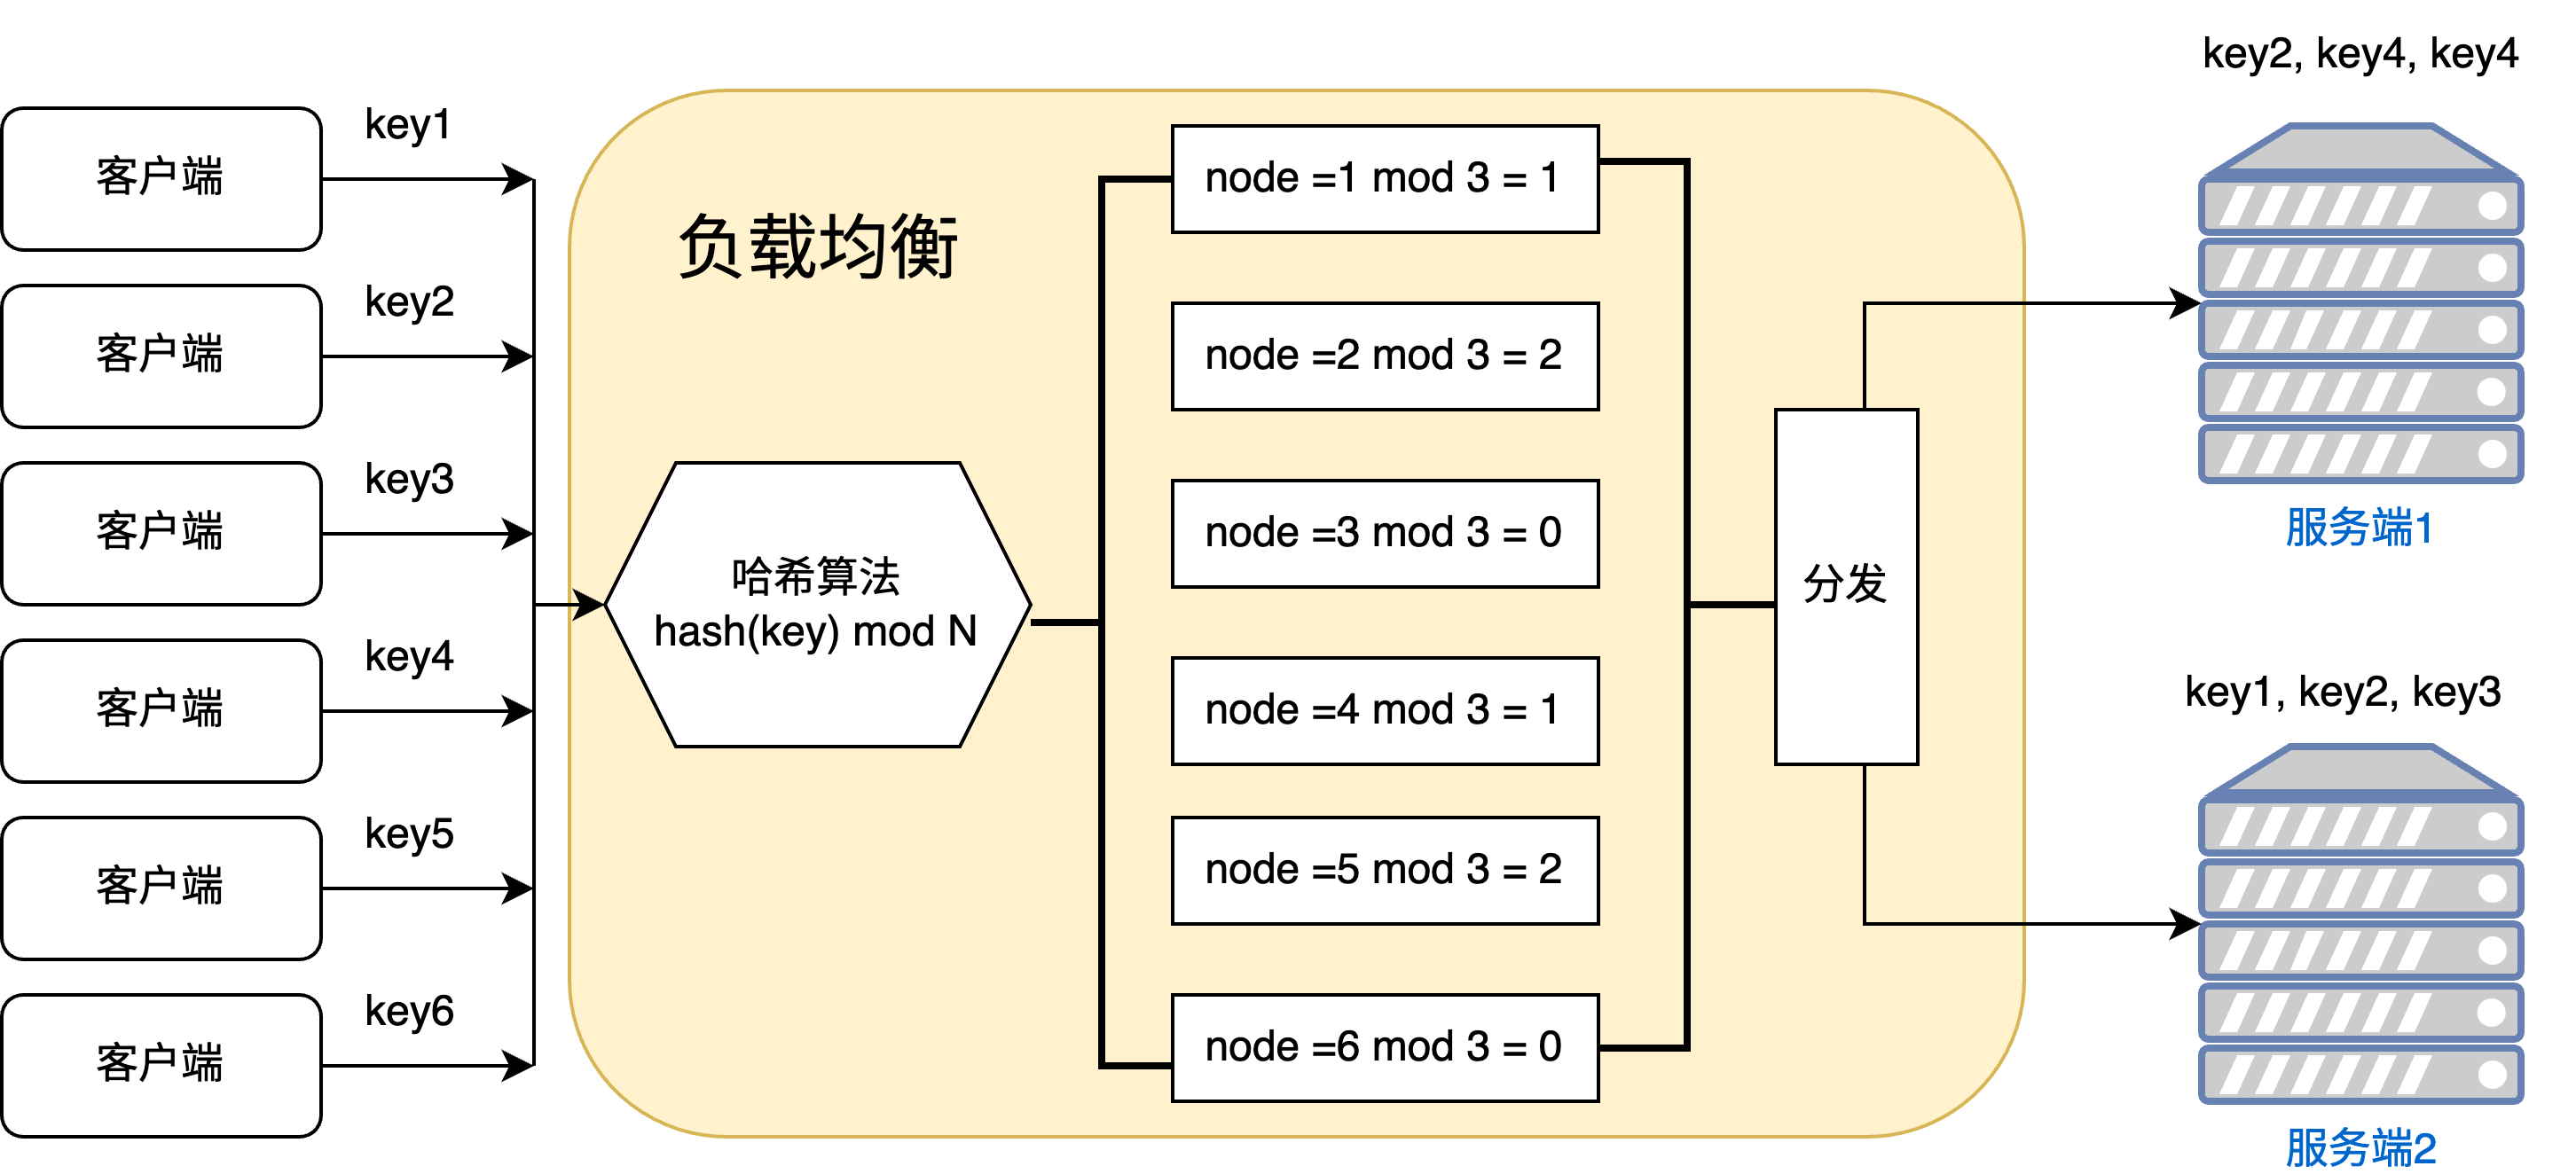
\includegraphics[width=\textwidth]{figures/hash-algo.png}
	\caption{Nginx 哈希算法拓扑图}
\end{figure}

Nginx通过使用IP哈希算法增强了客户端请求的处理效率。此算法取来源客户端的IP地址作为关键值(key),运用特定的哈希函数进行计算,然后根据得到的哈希结果将请求定向至集群中的相应服务器进行处理。
在实施过程中,将客户端IP地址的前三段作为输入参数进行哈希运算,确保具有相同前三段的IP地址能够一致性地被指派到同一台上游服务器。
完成哈希运算后,通过对得出的哈希值与集群中所有正常运行的服务器的总数执行模运算(取余数),从而确定应将请求分配到哪台服务器上。在这一过程中,如果请求持续失败次数超过20次,那么Nginx将转而采用加权轮询策略以分发任务请求。以下是配置Nginx使用IP哈希算法的示例。

\begin{lstlisting}
# IP-HASH 算法
upstream backend {
    ip_hash;
    server 127.0.0.14:80 max_fails=2 fail_timeout=10s;
    server 127.0.0.15:80 max_fails=2 fail_timeout=10s;
}
\end{lstlisting}

IP 哈希算法流程图如下所示。

\begin{figure}[htb]
	\centering
	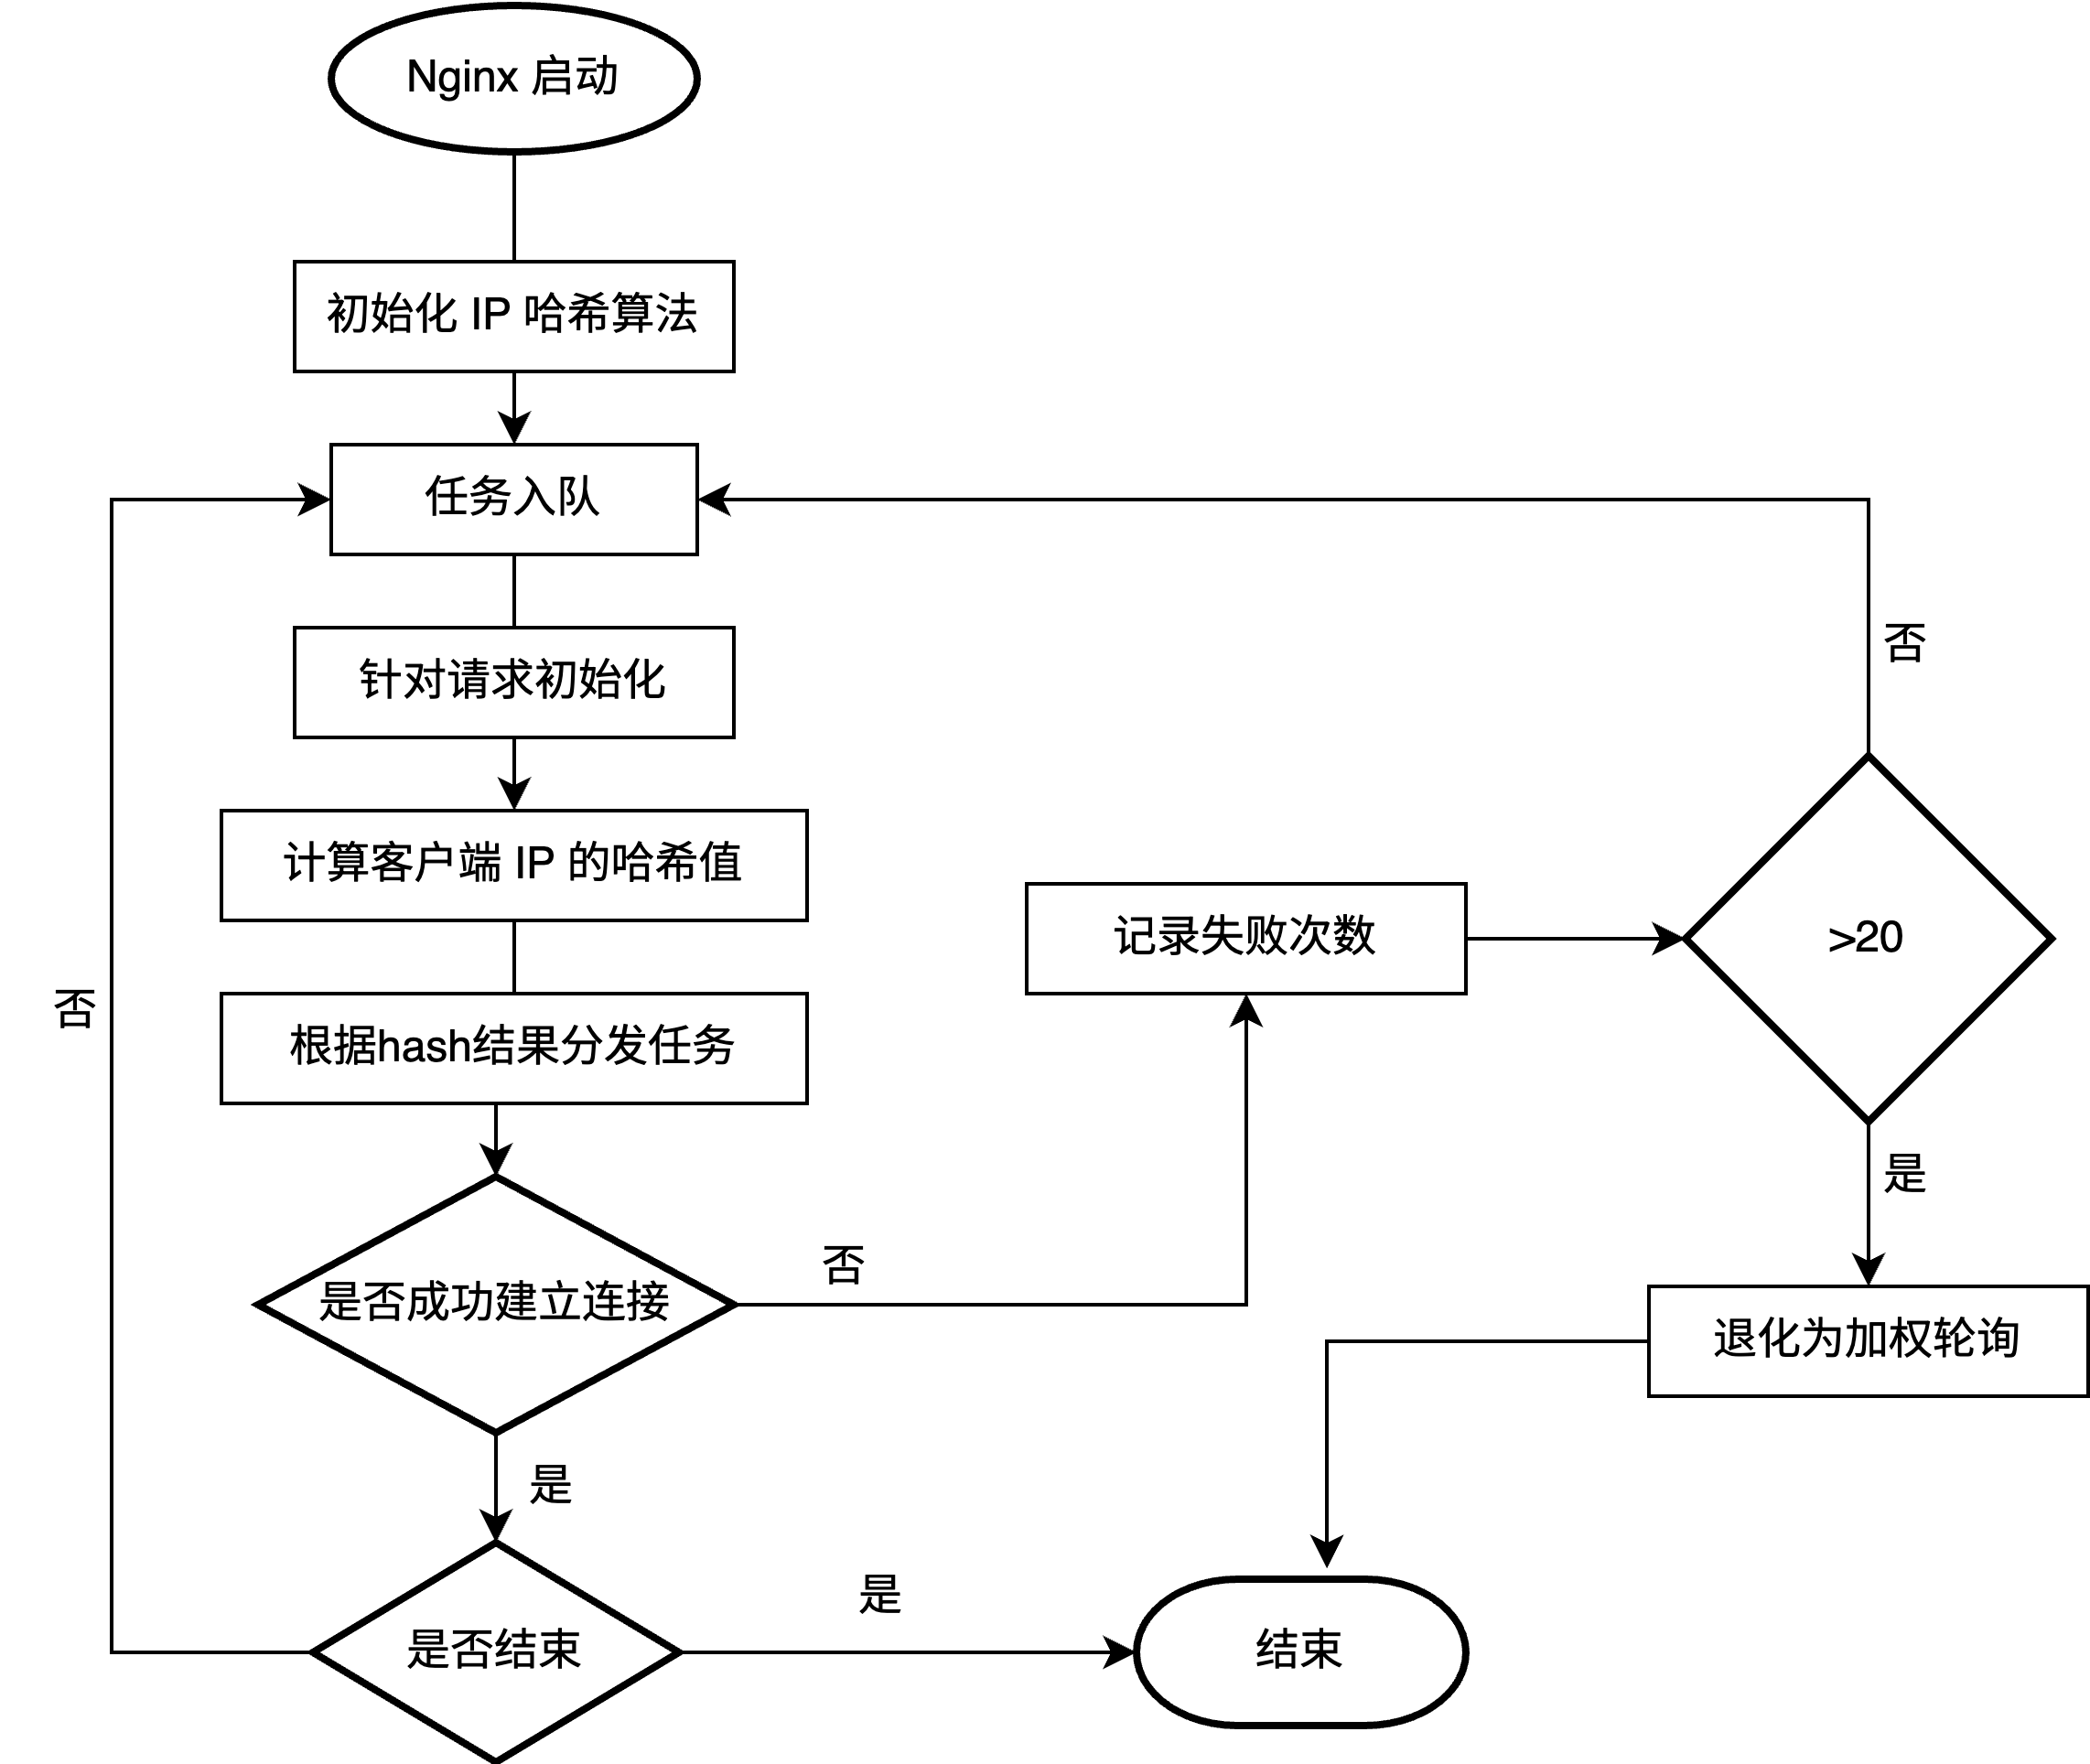
\includegraphics[width=\textwidth]{figures/hash-flowchart.png}
	\caption{Nginx IP 哈希算法流程图}
\end{figure}

IP 哈希算法有助于维持用户会话的连续性,原因在于来自同一IP的用户请求将被映射至同一服务器节点处理。
然而,当集群节点发生故障或有新节点加入集群时,需要重新进行哈希运算,这可能导致会话一致性问题。
在高并发的情况下,由于IP哈希算法未能考虑到不同资源的消耗情况,仍可能会导致服务器节点过载崩溃,同时其他节点资源处于空闲状态。
因此,任何无法完全洞悉集群节点实时负载的负载均衡算法,都很难保证节点不会过载或处于过度空闲状态。

在Nginx支持的众多负载均衡策略里,除了若干广为人知的默认调度算法,还包括一种称作“最小响应比算法”的高级调度机制。
其中,“fair”算法尤其引人注目,它在分配客户端请求过程中主要参考上游服务器的响应时长,优先考虑响应速度较快的服务器。
这一算法基于的核心思想是,响应时间较长的服务器可能面临较高的负载,因而在分配新的请求时宜赋予较低的优先权。
通过动态评估页面大小及其加载时间,Fair算法能够自适应地平衡负载,旨在最大程度减少用户的等待时长,从而在考量上游服务器性能差异方面提供了一种有效的解决方案。

然而,在处理高并发的场景下,该算法并未充分考虑网络拥堵等因素可能导致的响应时间延长,且仅依据响应时间来评估服务器负载情况存在一定局限性。这种单一维度的负载判断方法可能不足以全面准确地反映服务器的实际负载情况\cite{张艳肖2023基于Fair函数神经网络的厚度传感器输出特性分析}。

经过上面的对Nginx几种内置的负载均衡算法可以得知,静态负载均衡算法配置一遍比较简单,而且执行效率很好,一定程度上能够反应集群节点的负载性能。
而动态负载均衡则配置比较复杂,在不考虑多方面的情况下,不够准确可靠,但是相比于静态负载均衡能够更加实时的了解某一节点的性能状态,以至于能够让
负载均衡器更好的分配工作。于是本文将从机器学习和神经网络方面探究动态负载均衡中关于网络方面的优化,并分析结果加以与原来对比。

\section{本章小结}

本章主要阐述了常规负载均衡算法探究涉及的相关理论和技术。首先介绍了服务器集群的概念和分类,
同时确定了如何测量服务器剩余节点性能的标准。其次分析了负载均衡技术的意义与优势,在分析负载均衡类型的过程中
确认了要突破的方向。最后通过对于Nginx 源码的了解探究了 Nginx 的工作模式和进程模型,了解了常规的负载均衡算法以及实现,
明确了动态负载均衡算法的改进研究方向。
